\documentclass{article}

\usepackage[utf8]{inputenc}

\usepackage{amsmath, bm}
\usepackage{graphicx}
\usepackage{amssymb}
\usepackage{float}
\usepackage{caption}
\usepackage{subcaption}
\usepackage{hyperref}
\usepackage{tikz}
\usetikzlibrary{calc}
\usetikzlibrary{angles,quotes} % for pic
\usetikzlibrary{patterns,snakes}
\tikzset{>=latex} % for LaTeX arrow head

\usepackage[margin=0.5in]{geometry}

\setlength{\parskip}{\baselineskip}%
\setlength{\parindent}{0pt}%


% PULLEY
\def\r{0.05} % pulley small radius
\tikzset{
  pics/pulley/.style={
    code={
      \draw[pulcol,line width=0.6] (0,0) circle (#1);
      \draw[pulcol,thick] (0,0) circle (\r);
  }},
  pics/mount/.style args={#1:#2}{ % angle, length
    code={
      \draw[mount] (0,0)++(#1-90:0.9*\r) arc (#1-90:#1-270:0.9*\r) --++ (#1:#2) --++ (#1-90:1.8*\r) -- cycle;
  }},
  pics/weight/.style args={#1,#2,#3}{ % bottom width, top width, height
    code={
      \draw[mass] (0,0) -- (#2/2,0) -- (#1/2,-0.7*#3)
        |- (-#1/2,-#3) -- (-#1/2,-0.7*#3) -- (-#2/2,0) -- cycle;
      \path[mass] (0,0) -- (0,-#3) node[pos=0.52] {$m$};
  }},
  pics/pulley/.default=0.45,
}

\tikzstyle{vvec}=[->,vcol,thick,line cap=round]
\tikzstyle{ground}=[preaction={fill,top color=black!10,bottom color=black!5,shading angle=20},
                    fill,pattern=north east lines,draw=none,minimum width=0.3,minimum height=0.6]
\tikzstyle{metal}=[fill,top color=black!40,bottom color=black!20,shading angle=10]
\tikzstyle{mass}=[line width=0.6,black!30!black,fill=black!40!black!10,rounded corners=1,
                  top color=black!40!black!20,bottom color=black!40!black!10,shading angle=20]
\tikzstyle{pulcol}=[draw=black!30!black,%fill=blue!40!black!10
                    top color=black!40!black!20,bottom color=black!40!black!10,shading angle=20]
\tikzstyle{rope}=[black,thick,line cap=round]
\def\rope#1{ \draw[black,line width=1] #1; \draw[rope] #1; }
\tikzstyle{mount}=[blue!20!black,fill,top color=blue!20!black!70,bottom color=blue!20!black!40,shading angle=10] %,line width=1.8,line cap=round
%\tikzstyle{mount}=[color=black!60,line width=1.8,line cap=round]
%\tikzstyle{spring}=[line width=0.8,black!80,snake=coil,segment amplitude=5,segment length=5,line cap=round]
\tikzstyle{spring}=[thick,decorate,decoration={zigzag,pre length=0.3cm,post length=0.3cm,segment length=6}]

\pgfdeclarelayer{back} % to draw on background
\pgfsetlayers{back,main} % set order

\begin{document}

\title{Full Technical Report: 3F2 Inverted Pendulum Lab}
\author{lwp26}
\date{March 2024}
\maketitle 

\begin{abstract}
    \centering

\end{abstract}

\newpage

\section{Introduction}
% and purpose
Control of systems is essential  

\subsection{Purpose}
% talk about why this is important

\subsection{Objectives}
% list the objectives of the experiment

% analyse mechanical systems

\section{Theory}

\subsection{Inverted Pendulum Dynamical System}

\def\h{0.8}  % mass height
\def\w{0.8}  % mass width
\def\R{0.45}  % pulley radius
\begin{figure}[H]
    \centering
    \begin{tikzpicture}
        \def\H{0.4} % wall height
        \def\T{0.3} % wall thickness
        \def\W{2.6} % ground length
        \def\D{0.2} % ground depth
        \def\x{1.4} % mass width
        \def\pA{-\W+1.8*\R} % A pulley x position
        \def\pB{\W+1.8*\R} % B pulley x position
        \def\Rp{0.25} % pendulum radius
        \def\xp{1.0} % pendulum x position
        \def\L{1.8}  % pendulum length
        \def\wh{0.15} % wheel height
        \draw[ground] (\pA,0) rectangle (\pB,-\D);
        %\draw (0,\H) -- (0,0) -- (\W,0) --++ (0,-\D);
        \rope{(\x,\h/2 + \wh) -- (\pA,\h/2 + \wh) arc (90:270:\R) --++ (-\pA,0) coordinate (T)}
        \pic at (\pA,\h/2-\R + \wh) {pulley};
        \rope{(\x+\w,\h/2 + \wh) -- (\pB,\h/2 + \wh) arc (90:-90:\R) --++ (-\pB,0) coordinate (T)}
        \pic at (\pB,\h/2-\R + \wh) {pulley};
        \draw[mass] (\x,\wh) rectangle ++ (\w,\h);
        \draw[black, thick] (\x+\wh/2, \wh/2) circle (\wh/2);
        \draw[black, thick] (\x+\w-\wh/2, \wh/2) circle (\wh/2);
        \node[above] at (\x+\w/2,\h + \wh) {$M$};
        \draw[fill, black] (\x+\w/2, \h/2 + \wh) circle (0.05);
        \draw[black,line width=1.0] (\x+\w/2, \h/2 + \wh) coordinate (b) -- (\xp,-\L) coordinate (a) node[midway, left] {$l$};
        \draw[mass] (\xp,-\L) circle (\Rp) ++ (0,0) node {$m$};
        \draw[dashed] (b) -- (\x+\w/2,-\L) coordinate (c);
        %% arrows 
        \draw[<-|] (\x+\w/2,\h+0.6) -- (\pA,\h+0.6) node[midway, above] {$x$};
        \pic[draw, <-, "$\theta$", angle eccentricity=1.5, angle radius=1.2cm] {angle=a--b--c};
        \draw[->,thick] (\pA,0)++(180:1.5*\R) arc (180:90:1.5*\R) node[midway, above] {$T$};

    \end{tikzpicture}

    \caption{Inverted pendulum system.}
    \label{fig:inverted_pendulum}
\end{figure}

\begin{figure}[H]
  \centering

  \begin{tikzpicture}
    \def\H{0.6} % wall height
    \def\T{0.3} % wall thickness
    \def\W{0.8} % ground length
    \def\D{0.2} % ground depth
    \def\x{0.8} % mass x position
    \def\pA{1.8*\R} % pulley x position
    \def\Rp{0.25} % pendulum radius
    \def\xp{0.2} % pendulum x position
    \def\L{1.8}  % pendulum length
    %\draw (0,\H) -- (0,0) -- (\W,0) --++ (0,-\D);

    \pic at (\pA,\h/2-\R) {pulley};
    \draw[->,thick] (\pA,0)++(180:1.5*\R) arc (180:90:1.5*\R) node[midway, above] {$T$};
    \draw[->>,thick] (\pA,0)++(135:3.0*\R) arc (135:90:3.0*\R)  --++ (0.3, -0.05) node[midway, above] {$\ddot{x}/a$};
    \draw[->,thick] (\pA,-\R-0.05) -- (\pA+1.0,-\R-0.05) node[midway, below] {$F_c$};

    \begin{scope}[xshift=5cm]

      \draw[mass] (\x,0) rectangle ++ (\w,\h);
      \draw[fill, black] (\x+\w/2, \h/2) circle (0.05) ++ (0,0) node[left] {$P$};
      \draw[black,line width=1.0] (\x+\w/2, \h/2) coordinate (b) -- (\xp,-\L) coordinate (a) node[midway, left] {$l$};
      \draw[mass] (\xp,-\L) circle (\Rp) ++ (-0.2,0) node[left] {$Q$};

      %% arrows 
      \draw[<-|] (\x+\w/2,\h+0.5) -- (-1,\h+0.5) node[midway, above] {$x$};
      \draw[->,thick] (\x+\w,\h/2) -- (\x+\w+1.0, \h/2) node[midway, above] {$F_c$};
      \draw[->,thick] (\x,\h/2) -- (\x-1.0, \h/2) node[midway, above] {$F_f$};
      \draw[->,thick] (\x+\w/2, 0) -- (\x+\w/2, -1.5) coordinate (c) node[midway, right] {$Mg$};
      \draw[->,thick] (\xp, -\L-\Rp) --++ (0, -0.6) node[midway, right] {$mg$};
      \draw[->,thick] (\x+\w/2, \h) --++ (0, +1.2) node[midway, right] {$R$};


      \pic[draw, <-, "$\theta$", angle eccentricity=1.5, angle radius=1.2cm] {angle=a--b--c};

    \end{scope}

  \end{tikzpicture}
  \caption{Free body diagrams of the inverted pendulum system.}
  \label{fig:inverted_pendulum_fbd}

\end{figure}
The forces $F_c$, $F_f$ and $R$ are the cable tension, friction force and vertical reaction acting on mass $M$.
The frictional force is defined below
\begin{equation}
  F_f = F \text{sgn}(\dot{x}) \quad \text{where} \quad \text{sgn}(\dot{x}) = \begin{cases} 1 & \dot{x} > 0 \\ -1 & \dot{x} < 0 \\ \text{undefined for } \dot{x} = 0 & \end{cases}
\end{equation}
The vectors $\mathbf{r}_P$ and $\mathbf{r}_Q$ are the position vectors of masses $M$ and $m$ respectively.
\begin{equation}
  \mathbf{r}_P = x \mathbf{i} \quad \text{and} \quad \mathbf{r}_Q = (x-l\sin\theta) \mathbf{i} - l\cos\theta \mathbf{j}
\end{equation}
These positions can be differentiated to find the momentum $\mathbf{p}$ of the body.
\begin{equation}
  \mathbf{p} = \left[(M+m)\dot{x}-ml\dot{\theta}\cos\theta \right] \mathbf{i} + ml\dot{\theta}\sin\theta\mathbf{j}
  \label{eq:trolly_momentum}
\end{equation}
The angular momentum about the point P is given by
\begin{align}
  \mathbf{h}_P &= \sum_i m_i(\mathbf{r}_i - \mathbf{r}_p) \times \mathbf{p}_i \\
  &= m (\mathbf{r}_Q - \mathbf{r}_P) \times \dot{\mathbf{r}}_Q \\
  &= \left[ -ml^2\dot{\theta} + ml\dot{x}\cos\theta \right] \mathbf{k}
\end{align}
This can be differentiated and used with the equation below to find one of the equations of motion 
\begin{equation}
  \mathbf{Q}^{(e)} = \dot{\mathbf{h}}_P + \dot{\mathbf{r}}_P \times \mathbf{p}
\end{equation}
Here the only external force that does not pass through P is the weight of the pendulum bob $mg$ which is a distance $l\sin\theta$ from P,
and so the torque acts in the $+\mathbf{k}$ direction. The equation of motion is then
\begin{equation}
  mgl\sin\theta = ml\ddot{\theta} - ml\ddot{x}\cos\theta
  \label{eq:angular_momentum_deriv_eq}
\end{equation}
From differentiating the linear momentum $\mathbf{p}$ and from newtons second law;
\begin{equation}
  \dot{\mathbf{p}} = \left[F_c - F_f \right] \mathbf{i} + \left[ R - (m+M)g \right]\mathbf{j}
\end{equation}
From considering the unrestrained $\mathbf{i}$ direction the equation of motion is shown to be:
\begin{equation}
  (M+m)\ddot{x} - ml\ddot{\theta}\cos\theta + ml\dot{\theta}^2\sin\theta = F_c - F_f
  \label{eq:x_momentum_deriv_eq}
\end{equation}
However, the force in the cable $F_c$ is required to be in terms of the torque $T$ by the motor.
This is found from considering the angular momentum about the motors axis. The angular acceleration of the pulley is $\ddot{\alpha}$ and the radius of the pulley is $a$.
\begin{align}
  Q &= I\ddot{\alpha} \notag \\
  aF_c - T &= -I\frac{\ddot{x}}{a} \notag \\
  \implies F_c &= \frac{T}{a} - \frac{I}{a}\ddot{x}
\end{align}
This can be then substituted into equation \ref{eq:x_momentum_deriv_eq} and rearanged to give the equation of motion in terms of the torque $T$.
This is shown below along with a simplified form of equation \ref{eq:angular_momentum_deriv_eq}.

\begin{align}
  \left( 1 + \frac{M}{m} + \frac{I}{ma^2} \right) \ddot{x} &= \frac{T}{ma} - \frac{F}{m}\text{sgn}(\dot{x}) + l\cos\theta . \ddot{\theta} - l\sin\theta . \dot{\theta}^2 \label{eq:motion_1} \\
  l \ddot{\theta} &= \cos\theta \ddot{x} - g\sin\theta \label{eq:motion_2}
\end{align}

\subsection{State Space Model}

A linear state space model is given by the following equations
\begin{align}
  \mathbf{\dot{x}} &= \mathbf{Ax} + \mathbf{B}u \\
  \mathbf{y} &= \mathbf{Cx}
\end{align}
Where the state vector $\mathbf{x}$ is defined as a perturbation from an equilibrium point and the matricies are defined as follows,
\begin{equation}
  \mathbf{A}_{ij} = \frac{\partial f_i}{\partial x_j} \Bigr|_{\mathbf{x}=\mathbf{x}_e} \quad \mathbf{B}_{i} = \frac{\partial f_i}{\partial u} \Bigr|_{\mathbf{x}=\mathbf{x}_e}
\end{equation}

The Laplace transform of the state space model is taken and rearanged into a matrix of transfer functions for the system.

\begin{equation} 
  \frac{\mathbf{y}}{u} = \mathbf{C} (s\mathbf{I} - \mathbf{A}) ^{-1} \mathbf{B}
\end{equation}

\subsection{Controllability}

% waffle through controllability
% define controlability

A state space model is controllable if given initial and final states $\mathbf{x}(0)$ and $\mathbf{x}(t)$
then there exists an input signal $u$ that transfers from the initial to the final state in finite time $t$.

It can be shown from Cayley-Hamilton theorem that\dots 

\begin{equation}
  \mathbf{P} = \begin{bmatrix}
    \mathbf{B} & \mathbf{AB} & \cdots & \mathbf{A}^{n-1}\mathbf{B}
  \end{bmatrix}
\end{equation}

\subsection{Closed loop stability}
Given that the system is controllable, the poles can be arbitrarily assigned using closed loop feedback.
With feedback the new plant input is $u = w - \mathbf{Kx}$, where $\mathbf{K}$ is the control gain matrix.
This means that the closed loop transfer function is given by
\begin{equation}
  \frac{\mathbf{y}}{w} = \mathbf{C} (s\mathbf{I} - \mathbf{A} + \mathbf{KB}) ^{-1} \mathbf{B}
\end{equation}

The poles of the closed loop transfer function are given by the roots of the characteristic polynomial
\begin{equation}
  \text{det} \left( s\mathbf{I} - \mathbf{A} + \mathbf{KB} \right) = 0
  \label{eq:det_poly}
\end{equation}

All poles must have a positive real part for the system to be stable.
The poles are the roots of a polynomial which means the Routh-Hurwitz criteria can be used.

\subsubsection{Crane Model}

For the crane model the equilibrium point is at $\theta = 0$ and $\dot{\theta} = 0$.
This means that equations \ref{eq:motion_1} and \ref{eq:motion_2} can be linearised about this point to give the equations:
\begin{align}
  \left( 1 + \frac{M}{m} + \frac{I}{ma^2} \right) \ddot{x} &= \frac{T}{ma} - \left(\frac{F}{m}\right)\text{sgn}(\dot{x}) + l \ddot{\theta} \label{eq:crane_motion_1} \\
  l \ddot{\theta} &= \ddot{x} - g\theta \label{eq:crane_motion_2}
\end{align}
These can be solved to give the state space model of the system.
\begin{align}
  \frac{d}{dt} \dot{x} &= \frac{mg}{l\left(M+\frac{I}{a^2}\right)} l\theta + u - f \\
  \frac{d}{dt} \dot{l\theta} &= -\frac{g}{l}l\theta + u - f
\end{align}
Where torque input $u$, and friction disturbance $f$, are defined as follows
\begin{equation}
  u = \frac{T}{a\left(M+\frac{I}{a^2}\right)} \quad \text{and} \quad f = \left(\frac{F}{M + \frac{I}{a^2}} \right) \text{sgn} (\dot{x})
  \label{eq:ss_system_inputs}
\end{equation}
The state space equations are in a form of simple harmonic motion with natural frequencies shown below,
\begin{align}
  \omega_1^2 &= \frac{g}{l} \\
  \omega_0^2 &= \omega_1^2\left(1 + \frac{m}{M+\frac{I}{a^2}} \right)
\end{align}
This gives the final state space model of the system as

\begin{equation}
  \frac{d}{dt} 
  \begin{bmatrix}
     x \\ \dot{x} \\ l\theta \\ \dot{l\theta} \end{bmatrix} = \begin{bmatrix} 
      0 & 1 & 0 & 0 \\ 0 & 0 & \omega_1^2 - \omega_0^2 & 0 \\ 0 & 0 & 0 & 1 \\ 0 & 0 & -\omega_0^2 & 0 \end{bmatrix} \begin{bmatrix} 
        x \\ \dot{x} \\ l\theta \\ \dot{l\theta} \end{bmatrix} + \begin{bmatrix} 
          0 \\ 1 \\ 0 \\ 1 \end{bmatrix} (u - f)
\end{equation}

\subsubsection{Inverted Pendulum Model}

For the inverted pendulum model the linearization is about the point $\theta = \pi$ and $\dot{\theta} = 0$.
The same quations of motion, \ref{eq:motion_1} and \ref{eq:motion_2}, are substituted with $\theta = \pi - \phi$.
\begin{align}
  \left( 1 + \frac{M}{m} + \frac{I}{ma^2} \right) \ddot{x} &= \frac{T}{ma} - \frac{F}{m}\text{sgn}(\dot{x}) - l\sin\phi . \ddot{\phi} - l\cos\phi . \dot{\phi}^2 \\
   - l \ddot{\phi} &= \sin\phi \ddot{x} - g\cos\phi
\end{align}
The new states become $\mathbf{x} = \left[ x \quad \dot{x} \quad l\phi \quad l\dot{\phi} \right]^T$

linearising equations \ref{eq:motion_1} and \ref{eq:motion_2} yield the following:
\begin{align}
  \left( 1 + \frac{M}{m} + \frac{I}{ma^2} \right) \ddot{x} &= \frac{T}{ma} - \left(\frac{F}{m} \right)\text{sgn}(\dot{x}) + l \ddot{\phi} \label{eq:invp_motion_1} \\
  l \ddot{\phi} &= \ddot{x} + g\phi \label{eq:invp_motion_2}
\end{align}

The states can be substituted and solved for the state space model in terms of the same input $u$ and disturbance $f$ as the crane model defined in equation \ref{eq:ss_system_inputs}.

\begin{equation}
  \frac{d}{dt} 
  \begin{bmatrix}
     x \\ \dot{x} \\ l\phi \\ \dot{l\phi} \end{bmatrix} = \begin{bmatrix} 
      0 & 1 & 0 & 0 \\ 0 & 0 & \omega_0^2 - \omega_1^2 & 0 \\ 0 & 0 & 0 & 1 \\ 0 & 0 & \omega_0^2 & 0 \end{bmatrix} \begin{bmatrix} 
        x \\ \dot{x} \\ l\phi \\ \dot{l\phi} \end{bmatrix} + \begin{bmatrix} 
          0 \\ 1 \\ 0 \\ 1 \end{bmatrix} (u - f)
\end{equation}

\subsection{Closed loop control}


\subsubsection{Crane}

From equation \ref{eq:det_poly} the closed loop characteristic polynomial of the crane model is given by
\begin{equation}
  s^{4} + \left(k_{2} + k_{4}\right) s^{3} + \left(k_{1} + k_{3} + \omega_{0}^{2}\right) s^{2} + k_{2} \omega_{1}^{2} s + k_{1} \omega_{1}^{2}
  \label{eq:crane_poly}
\end{equation}
Application of the Ruth Hurwitz criteria gives the following conditions for stability
\begin{align}
  k_{2} + k_{4} &> 0 \\
  k_{1} + k_{3} + \omega_{0}^{2} &> 0 \\
  k_{2} \omega_{1}^{2} &> 0 \\
  \left(k_{3} + \omega_{0}^{2} - \omega_{1}^{2}\right) k_{2}^{2} + \left(- k_{1} k_{4} + k_{3} k_{4} + k_{4} \omega_{0}^{2}\right) k_{2} -  k_{1} k_{4}^{2} &> 0
\end{align}

At the point of marginal stability $s = \pm j\hat{\omega}$.
From substituting this into the characteristic polynomial \ref{eq:crane_poly} and considering both real and imaginary coefficients the following equations are found

\begin{align}
    - \hat{\omega}^{3} \left(k_{2} + k_{4}\right) + k_{2} \omega_{1}^{2} \hat{\omega}  &= 0 \\
    \hat{\omega}^{4} - \left(k_{1} + k_{3} + \omega_{0}^{2}\right)\hat{\omega}^{2} + k_{1} \omega_{1}^{2} &= 0
\end{align}

The first equation can be solved for the frequency $\hat{\omega}$ and substituted into the second equation to give:
\begin{align}
  \begin{gathered}
    \hat{\omega} = \sqrt{\frac{k_2}{k_2 + k_4}} \omega_1 \label{eq:marginal_stability_frequency}\\
    \frac{\omega_1^2}{(k_2+k_4)^2} \left( \left(k_{3} + \omega_{0}^{2} - \omega_{1}^{2}\right) k_{2}^{2} + \left(- k_{1} k_{4} + k_{3} k_{4} + k_{4} \omega_{0}^{2}\right) k_{2} -  k_{1} k_{4}^{2} \right) = 0
  \end{gathered}
\end{align}
The second result shows that the last condition for stability becomes an equality at the point of marginal stability.
The value of $k_2$ can be found by solving this equation and the solution is shown below.

\begin{equation}
  k_2 = \frac{k_{4} \left(k_{1} - k_{3} - \omega_{0}^{2} \pm \sqrt{k_{1}^{2} + 2 k_{1} k_{3} + 2 k_{1} \omega_{0}^{2} - 4 k_{1} \omega_{1}^{2} + k_{3}^{2} + 2 k_{3} \omega_{0}^{2} + \omega_{0}^{4}}\right)}{2 \left(k_{3} + \omega_{0}^{2} - \omega_{1}^{2}\right)}
\end{equation}
When this solution is substituted back into the characteristic polynomial

\subsubsection{Inverted Pendulum}

From equation \ref{eq:det_poly} the closed loop characteristic polynomial of the inverted pendulum model is given by

\begin{equation}
  s^{4} + \left(k_{2} + k_{4}\right) s^{3} + \left(k_{1} + k_{3} - \omega_{0}^{2}\right) s^{2} -  k_{2} \omega_{1}^{2} s -  k_{1} \omega_{1}^{2}
  \label{eq:pendulum_poly}
\end{equation}

Application of the Ruth Hurwitz criteria gives the following conditions for stability
\begin{align}
  k_{2} + k_{4} &> 0 \\
  k_{1} + k_{3} - \omega_{0}^{2} &> 0 \\
  - k_{2} \omega_{1}^{2} &> 0 \\
  \left(- k_{3} + \omega_{0}^{2} - \omega_{1}^{2}\right) k_{2}^{2} + \left(k_{1} - k_{3} + \omega_{0}^{2}\right) k_{4} k_{2} + k_{1} k_{4}^{2} &> 0
\end{align}

At the point of marginal stability $s = j\hat{\omega}$.
From substituting this into the characteristic polynomial \ref{eq:pendulum_poly} and considering both real and imaginary coefficients the following equations are found

\begin{align}
  - \hat{\omega}^{3} \left(k_{2} + k_{4}\right) - \hat{\omega} k_{2} \omega_{1}^{2} &= 0\\
  \hat{\omega}^{4} - \hat{\omega}^{2} \left(k_{1} + k_{3} - \omega_{0}^{2}\right) - k_{1} \omega_{1}^{2} &= 0
\end{align}
This gives the same frequency as the crane model \ref{eq:marginal_stability_frequency}. This is substituted back into the second equation to give:
\begin{equation}
  \frac{\omega_1^2}{(k_2 + k_4)^2} \left( \left(- k_{3} + \omega_{0}^{2} - \omega_{1}^{2}\right) k_{2}^{2} + \left(k_{1} - k_{3} + \omega_{0}^{2}\right) k_{4} k_{2} + k_{1} k_{4}^{2} \right) = 0
\end{equation}
This is again the same as the last condition for stability becoming an equality at the point of marginal stability.
The value of $k_2$ at the point of marginal stability is found by solving this equation and the solution is shown below.

\begin{equation}
  k_2 = \frac{k_{4} \left(k_{1} - k_{3} - \omega_{0}^{2} - \sqrt{k_{1}^{2} + 2 k_{1} k_{3} + 2 k_{1} \omega_{0}^{2} - 4 k_{1} \omega_{1}^{2} + k_{3}^{2} + 2 k_{3} \omega_{0}^{2} + \omega_{0}^{4}}\right)}{2 \left(k_{3} + \omega_{0}^{2} - \omega_{1}^{2}\right)}
\end{equation}

\subsubsection{Eigenvalue Sensitivity}

The roots of a polynomial can be very sensitive to coefficients, particularly when roots are nearly repeated.
This is shown by considering the polynomial
\begin{equation}
  d(s) = (s+k)^4 + \epsilon k^4
\end{equation}

\begin{figure}[H]
  \centering
  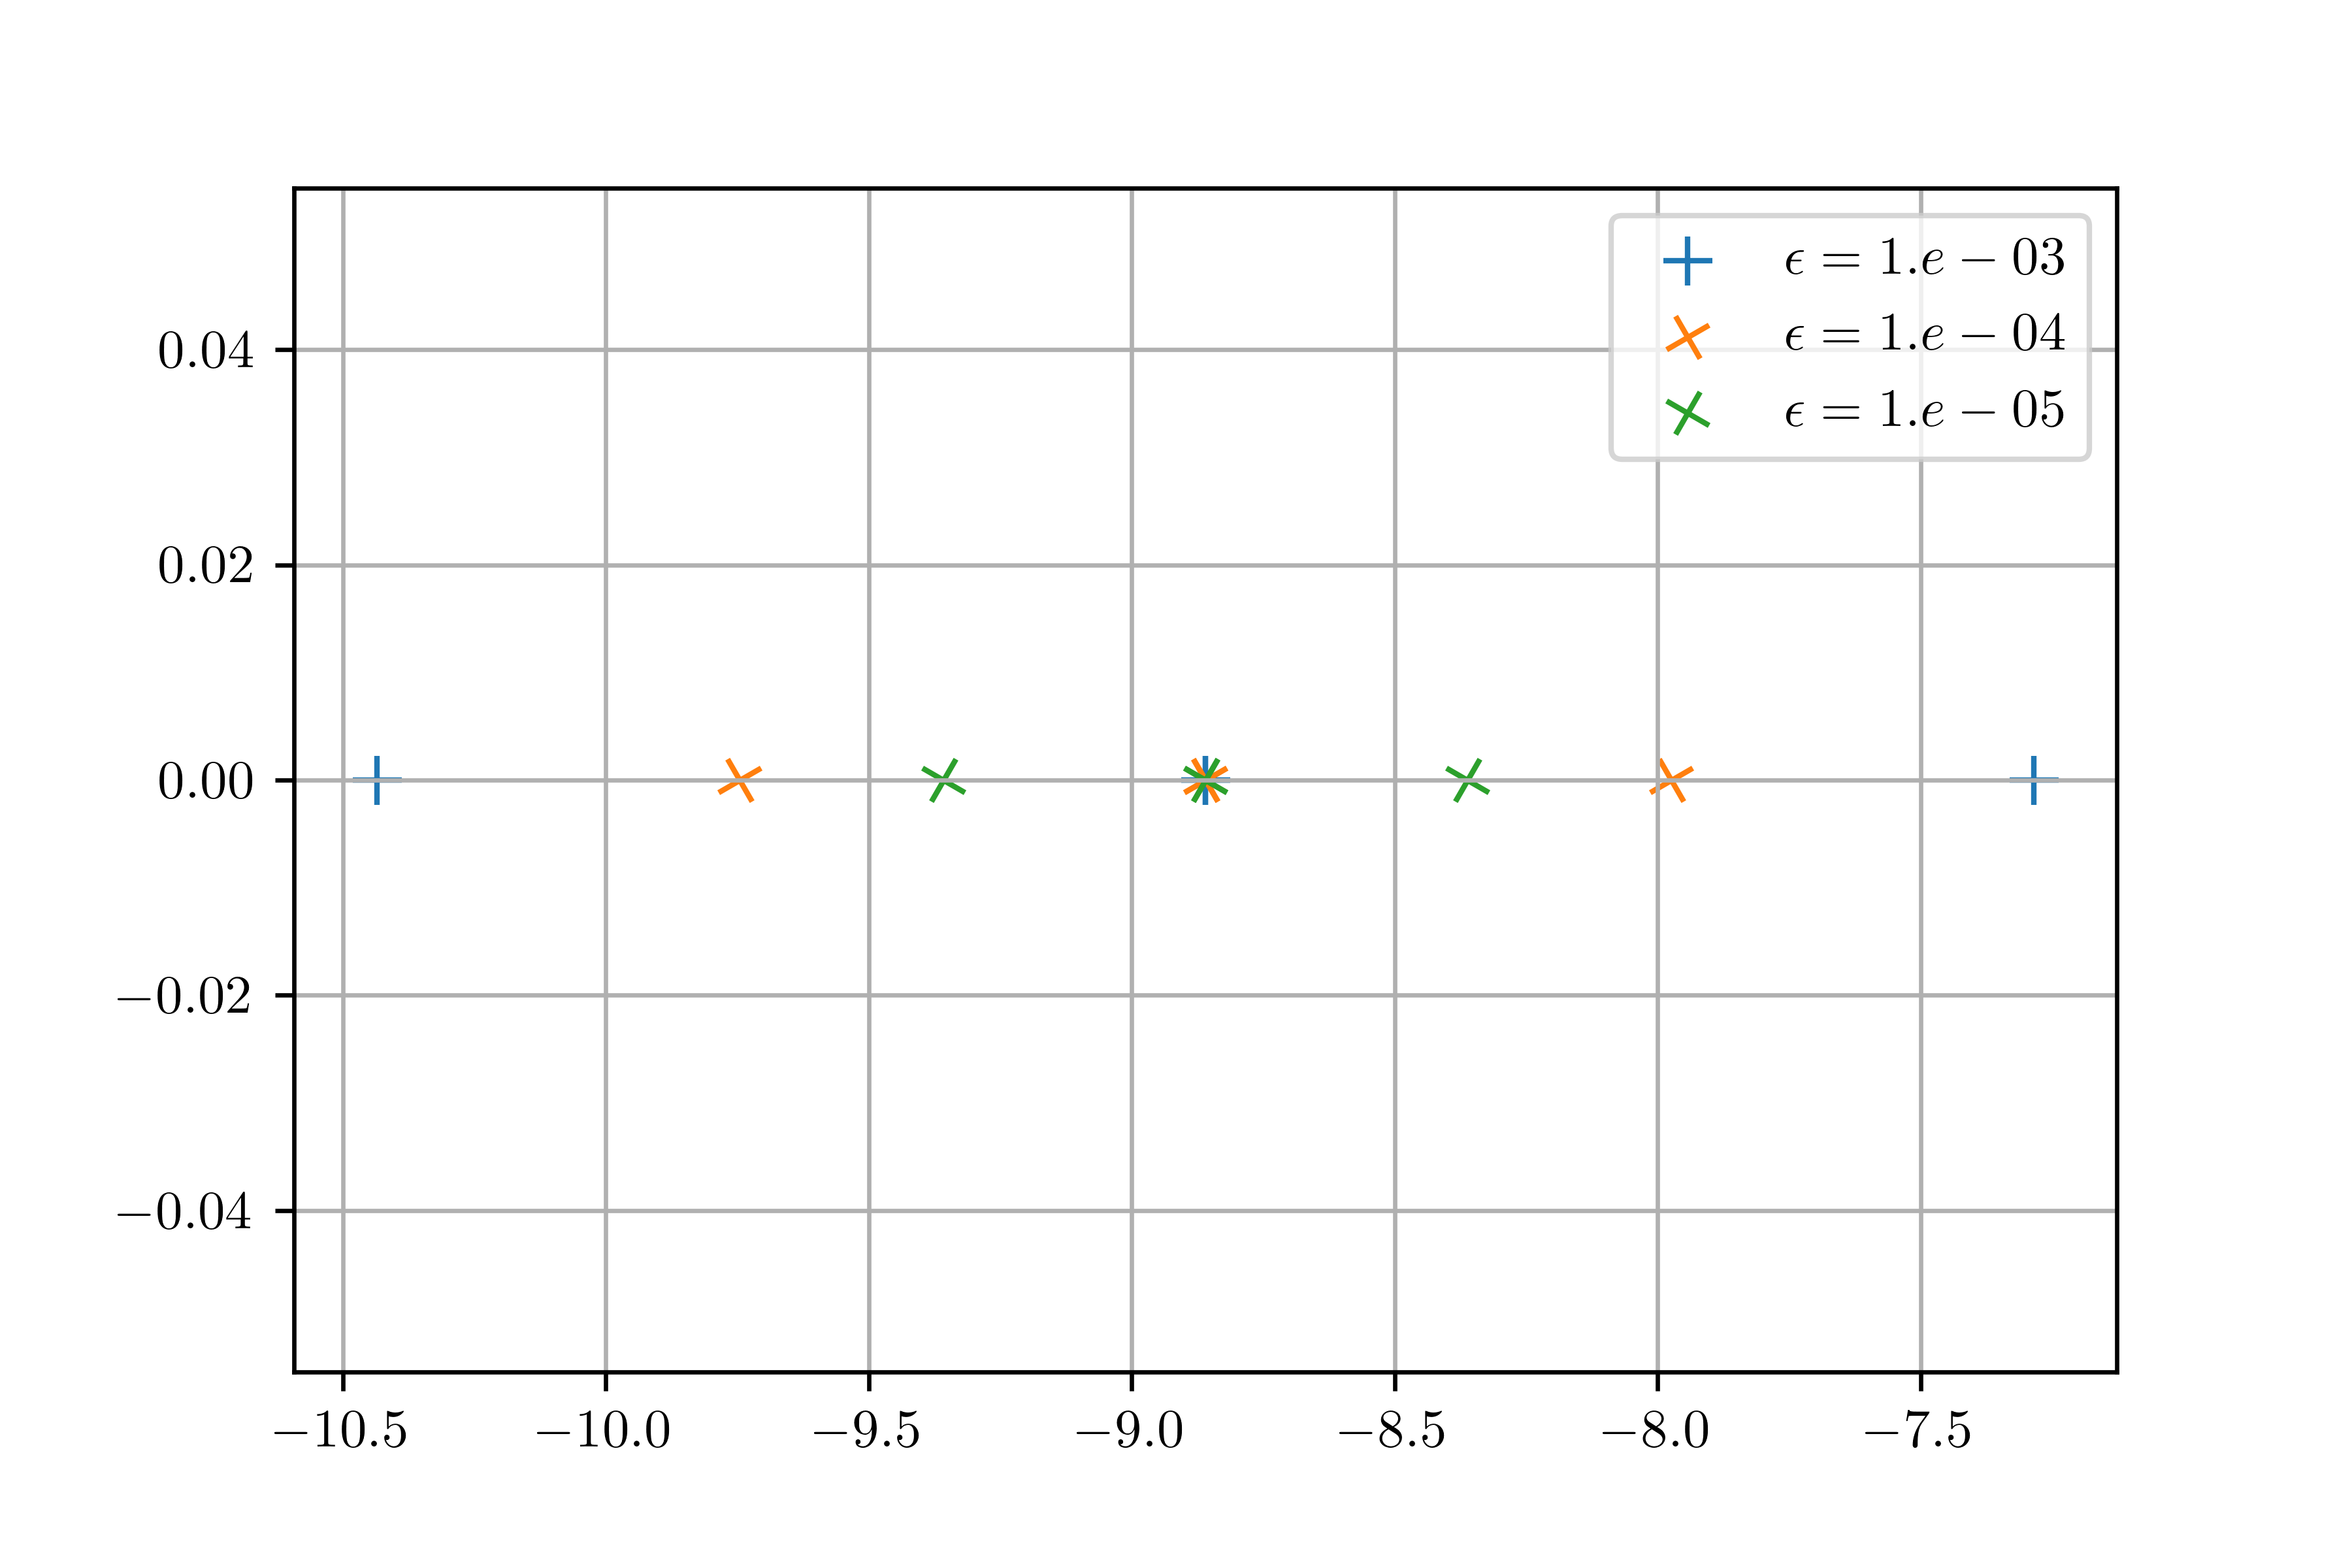
\includegraphics[width=0.6\textwidth]{figures/pole_sensitivity.png}
  \caption{}
  \label{fig:pole_sensitivity}
\end{figure}

\subsection{Nonlinear Friction term}
So far we have only considered linear theory, however the sign function in the friction term $f$ cannot be linearised.
The describing function method can be used to find the frequency-response function for
the nonlinear friction.

Suppose that $\dot{x} = E\text{sgn}(\omega t)$ then the $sgn(\omega t)$ can be expanded into a Fourier series seen below.

\begin{equation}
  \text{sgn}(\omega t) = \frac{4}{\pi}\sum_{n=0}^{\infty} \frac{\sin((2n+1)\omega t)}{2n+1}
\end{equation}

\subsection{Linear Quadratic Regulator}

The cost function associated with optimal control

\begin{equation}
  J = \int_0^\infty \left( \mathbf{x}^T \mathbf{Q} \mathbf{x} + \mathbf{u}^T \mathbf{R} \mathbf{u} \right) dt
\end{equation}

\subsubsection{Optimal Performance Evaluation}

The real world performance of the LQR determined system gains can be observed by measuring the input power and the response.

\section{Method}

\subsection{Apparatus}


\subsection{Procedure}


\subsection{Uncertainty}


\section{Results}

\subsection{Crane}

\begin{figure}[H]
  \centering
  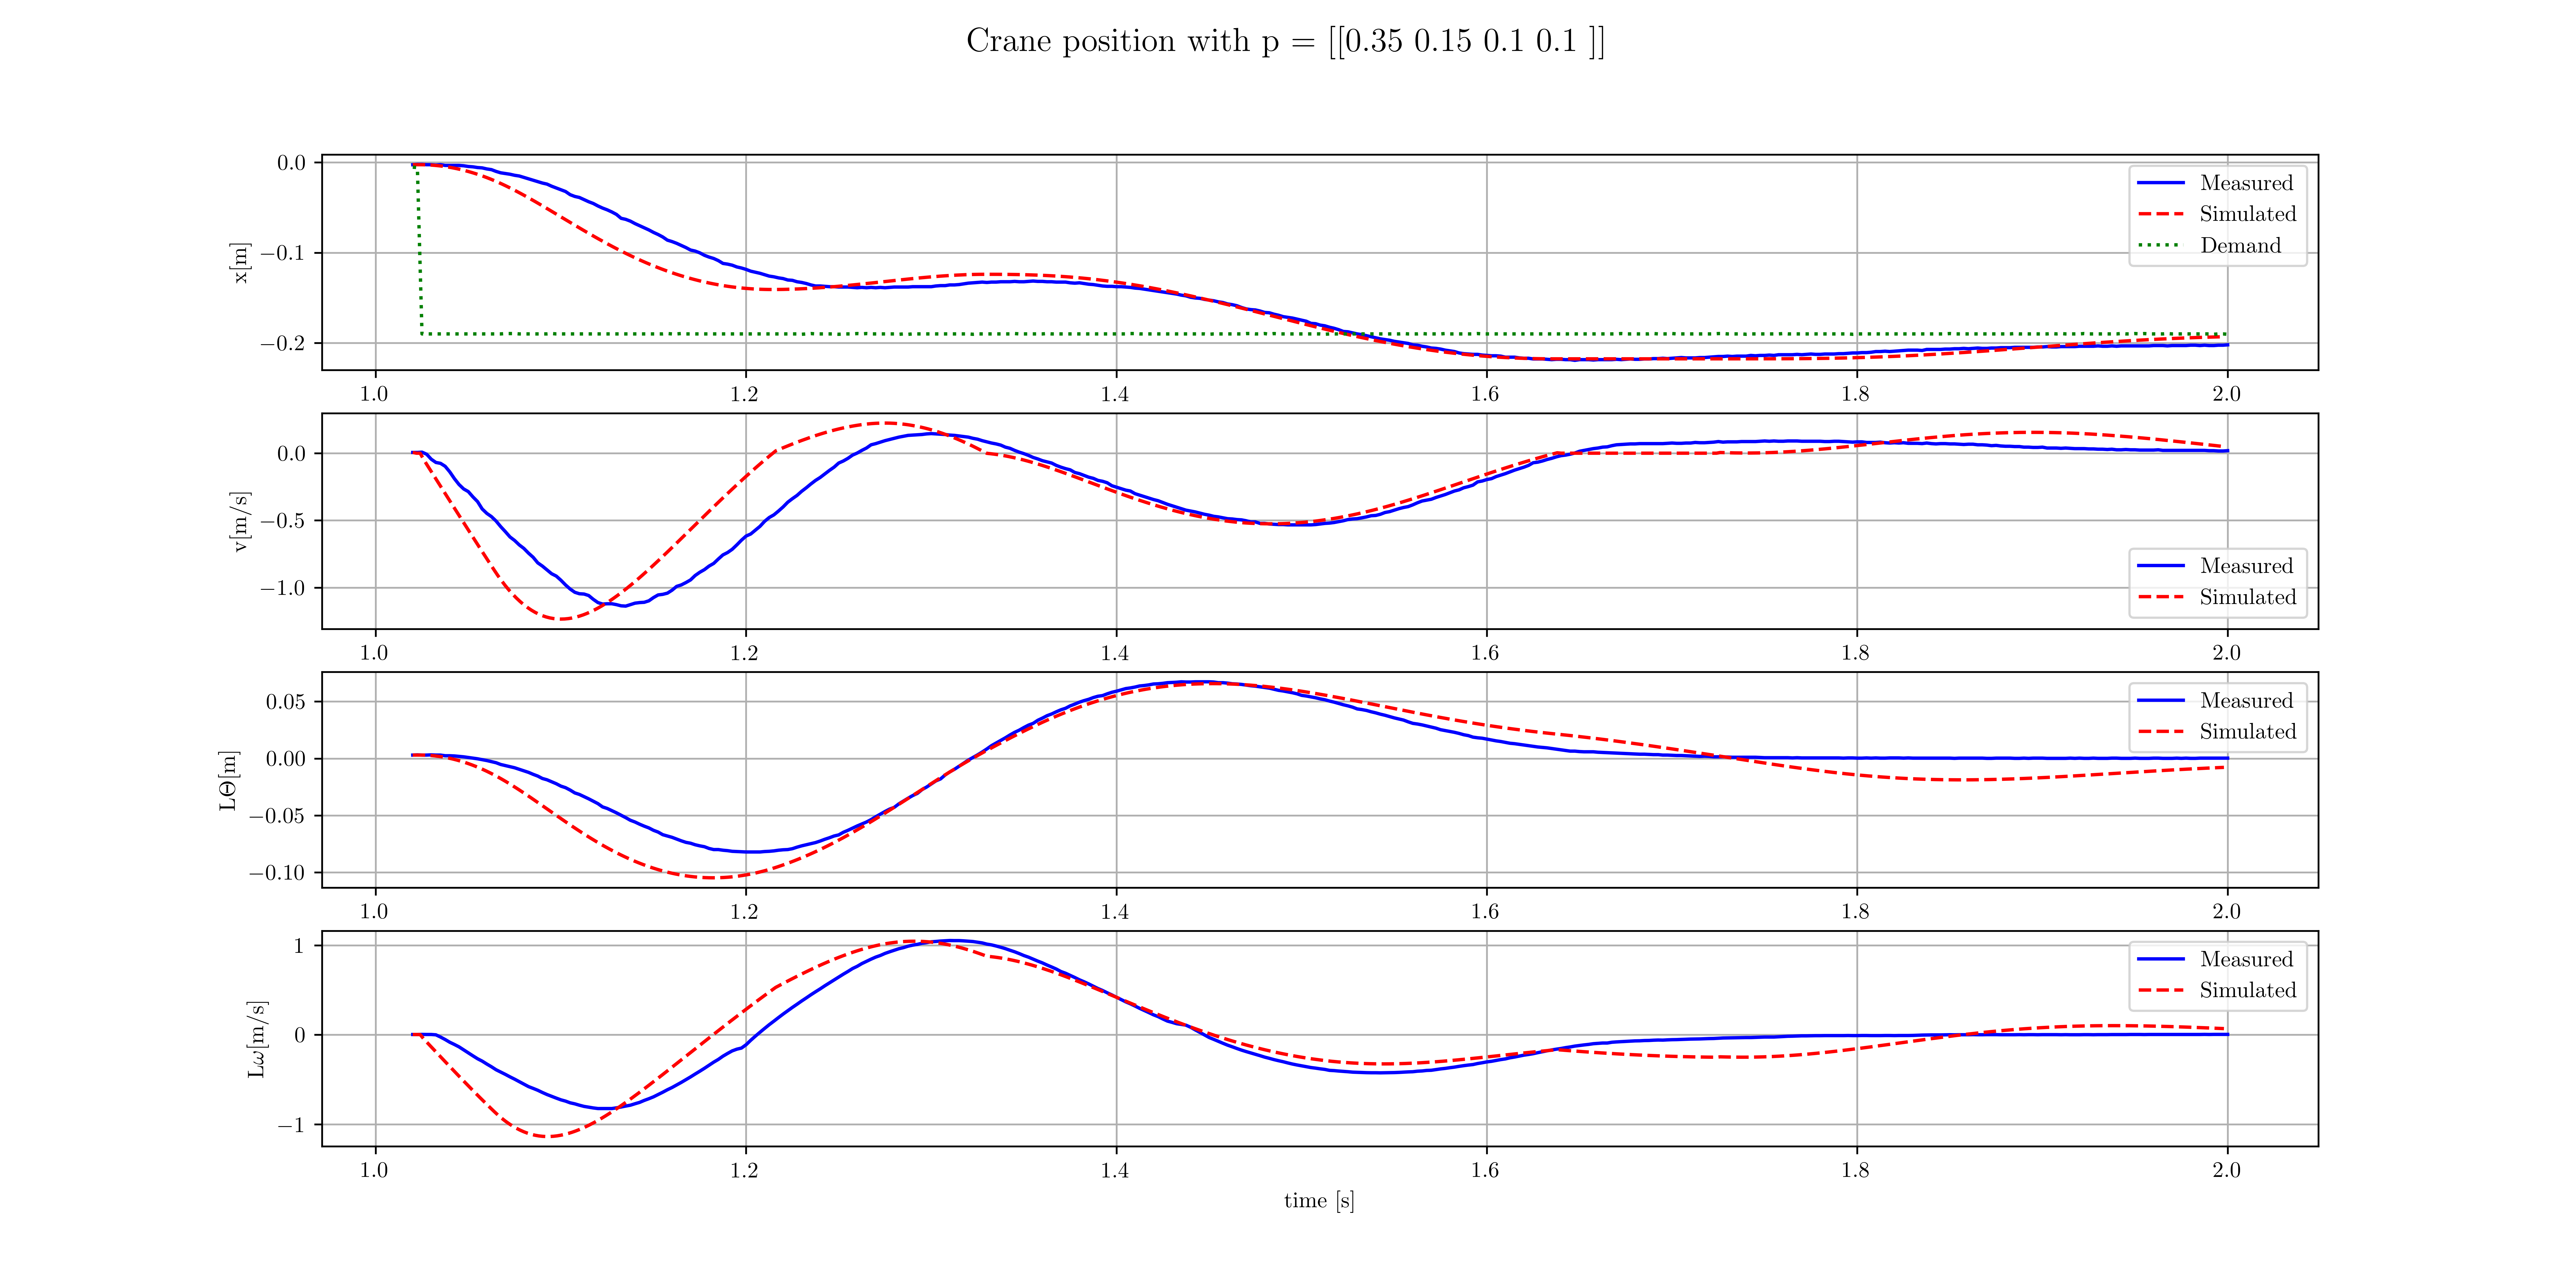
\includegraphics[width=0.99\textwidth]{figures/3.3.png}
  \caption{}
  \label{fig:exp3.3}
\end{figure}

From carriage velocity, the time for a period was measured at 0.36s which gives a frequency of 17.45 rad/s.
The system has high damping where the amplitude of carriage velocity halved over about 1 period, giving a damping ratio of $\zeta \approx 0.11$.

Calculated closed loop pole locations are: $[-3.89861823 \pm 18.69316043j, -2.16928301 \pm 6.46486529j]$
These indicate a highly damped system with frequency responses of 18.7 and 6.5 rad/s and corresponding damping ratios of ~0.208 and ~0.336.

The observed response is consistent with the calculated pole locations.

There is a small discrepency between the simulated and observed response. This is due to uncertainty in system parameters rather than numerical error in the verlet integrator method.
Uncertainty in the system parameters include the sensor constants, amplifier gains, friction coefficients, mass and moments of inertia of the system.


\begin{figure}[H]
  \centering
  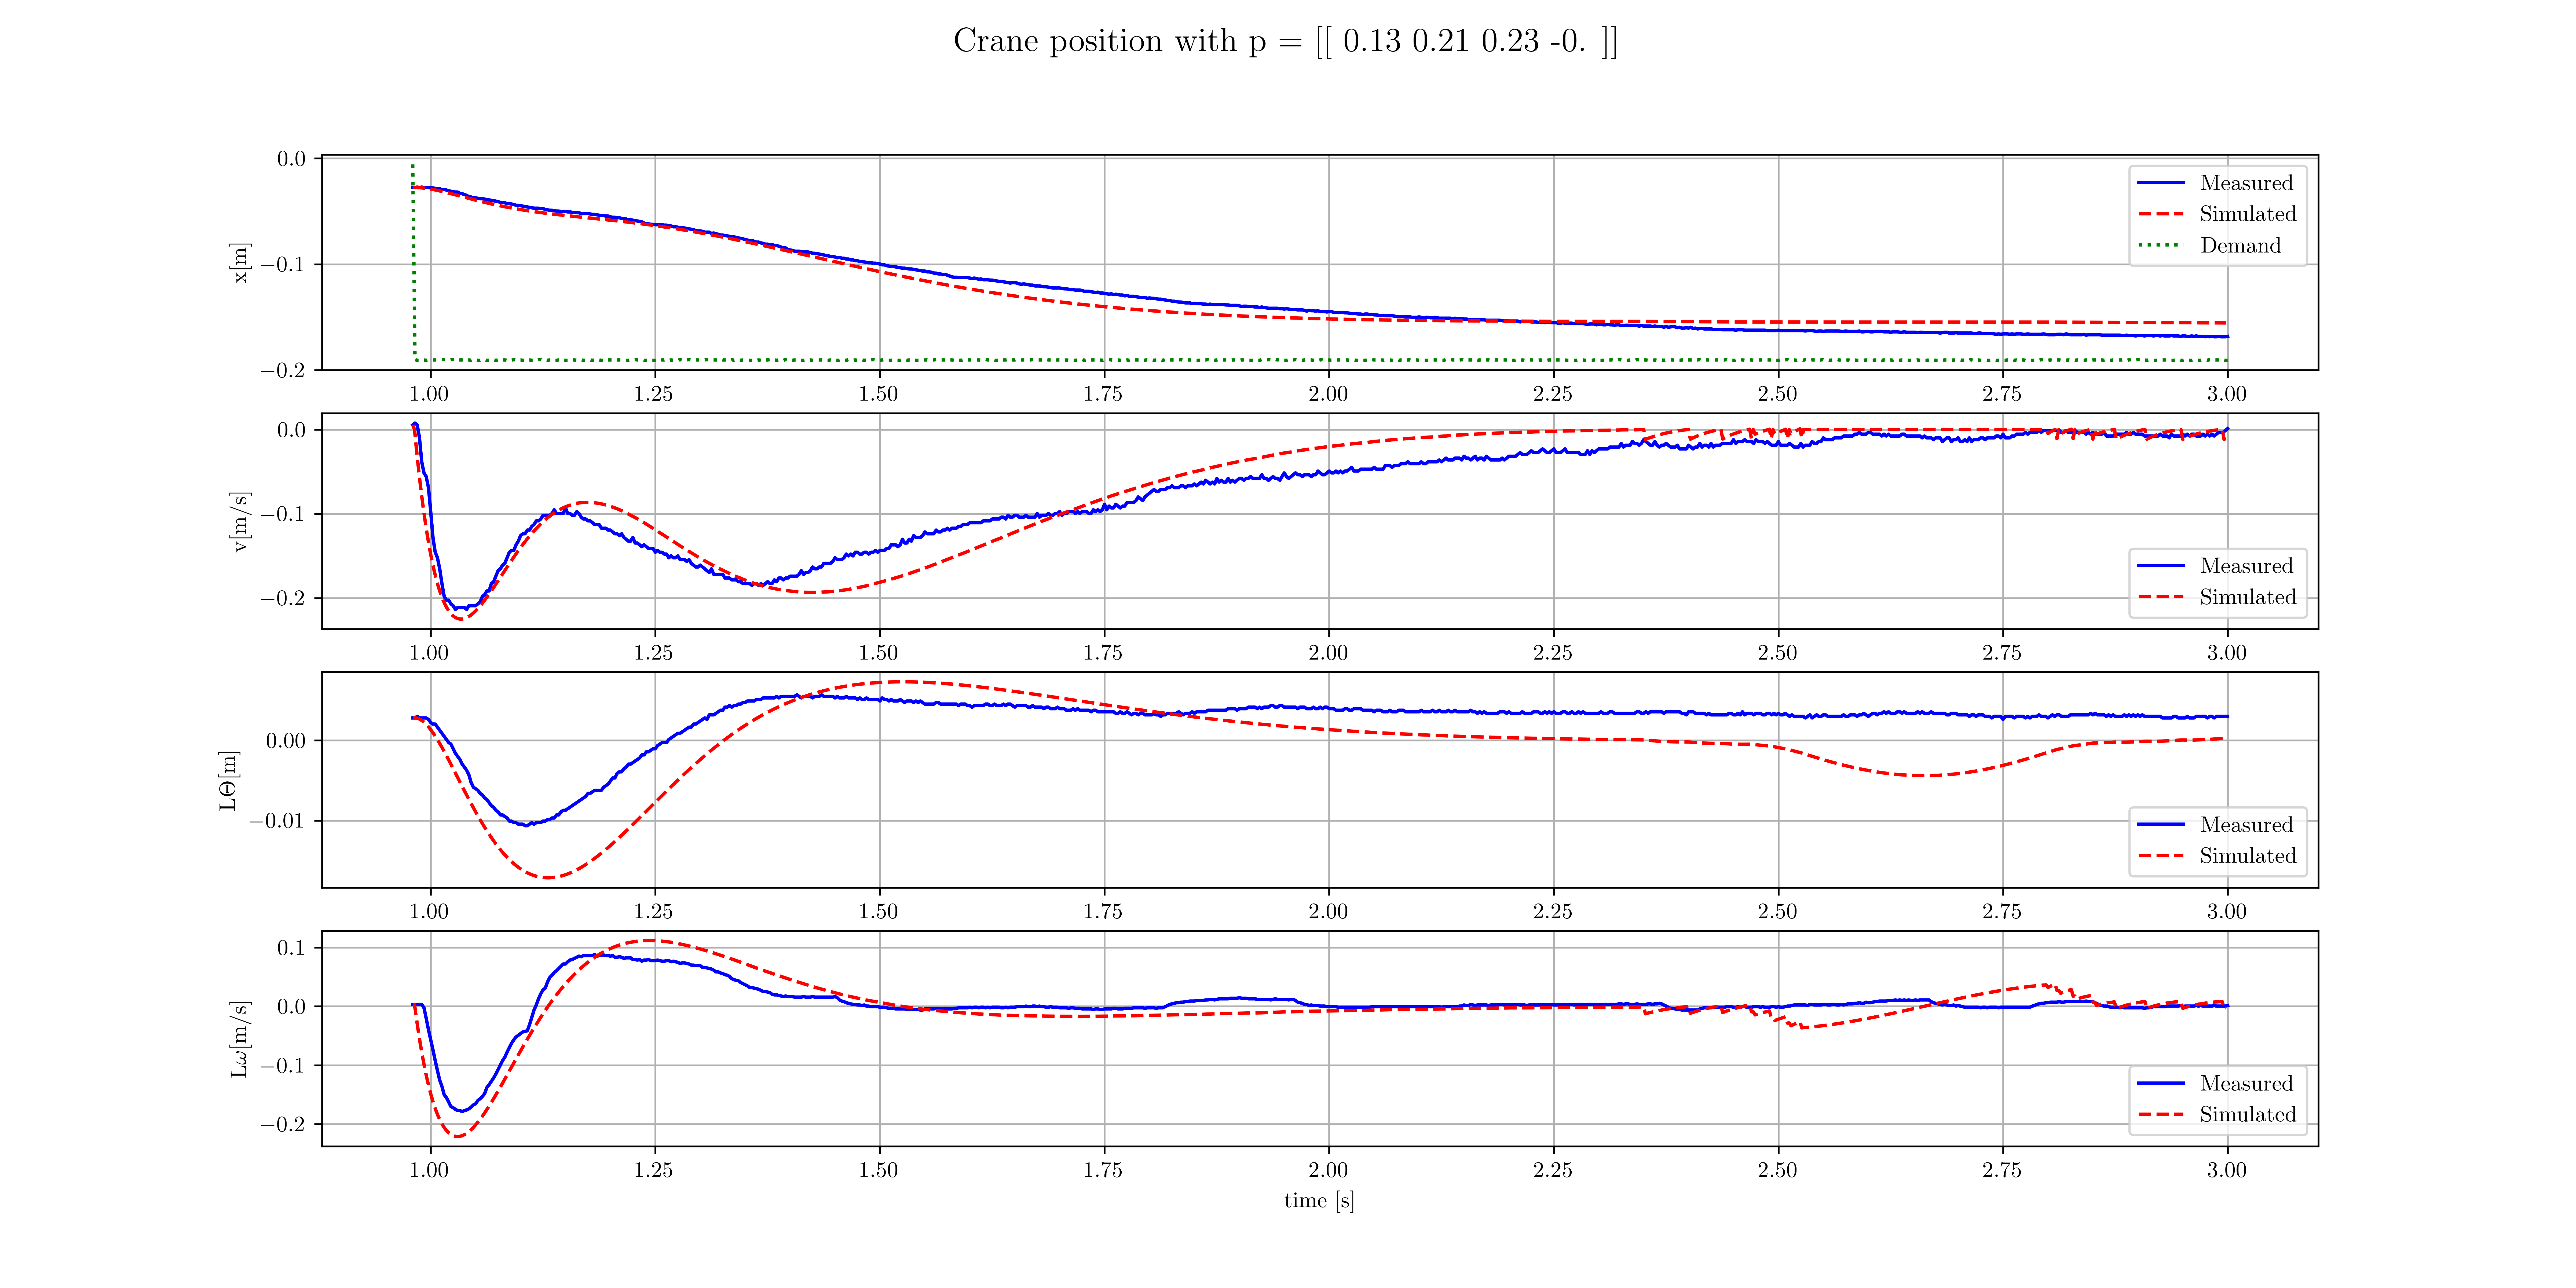
\includegraphics[width=0.99\textwidth]{figures/3.4a.png}
  \caption{All poles at $-\omega_1 = -\sqrt{78.5}$}
  \label{fig:exp3.4a}
\end{figure}

After carefully calculating the poles using $k_1 = \omega_1^2$, $k_2 = 4\omega_1$, $k_3 = 5\omega_1^2 - \omega_0^2$ and finally $k_4 = 0$ </br>
And converting using scale factors shown in the appendix A7, the gains $p_i$ were found to be $[ 0.13,  0.21,  0.23, 0.  ]$ </br>

The poles, however, were calculated from these values as $[-12.45360996 \pm 6.46216554j, -4.89083448 \pm 2.84116008j]$

This shows that the poles are not consistent with the target pole position. </br>
This may be due to the fact that the locations of poles are very sensitive to the coefficients of the closed loop characteristic polynomial.
This is especially true for repeated poles, which is the case here.

\begin{figure}[H]
  \centering
  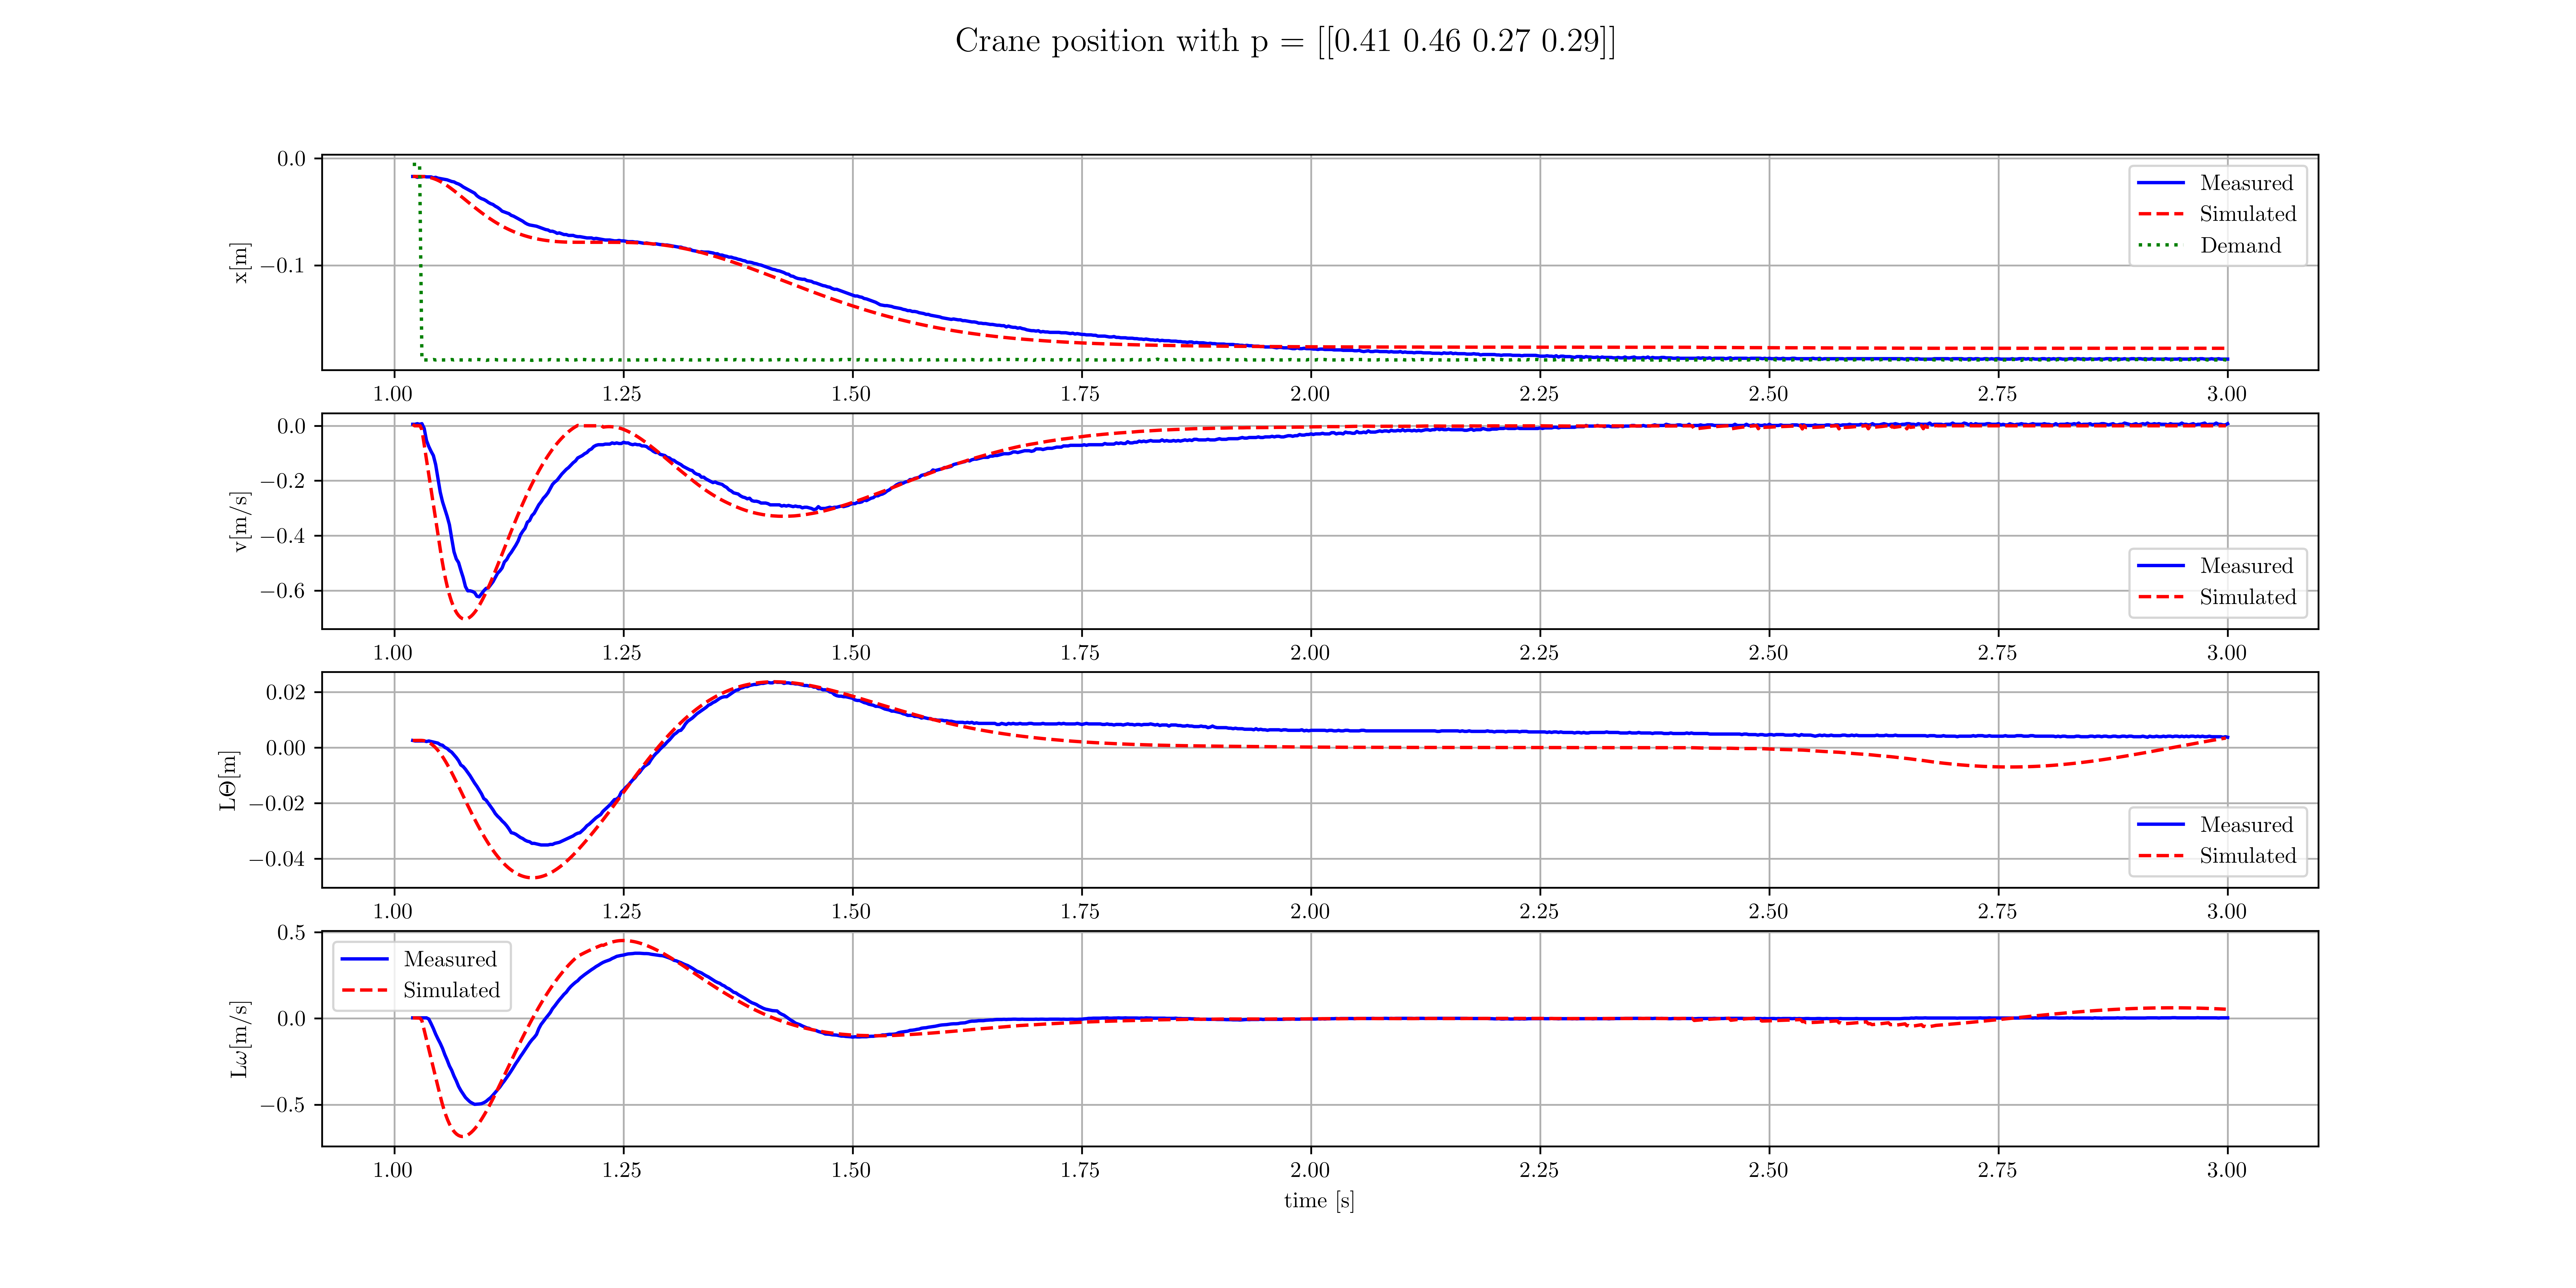
\includegraphics[width=0.99\textwidth]{figures/3.4b.png}
  \caption{Poles at $-\alpha, -\beta, -\omega \pm j\omega$ where $\alpha = 10; \beta = 10; \omega = 10$}
  \label{fig:exp3.4b}
\end{figure}

Chosen Values </br>
$\alpha = 10; \beta = 10; \omega = 10$

The calculated values of P are $[0.41284404 0.46282964 0.27212883 0.28834576]$ </br>
The poles are $[-10.0 \pm 10.0j, -10.0\pm 1.08564988\times 10^{-6}j ]$ which is very close to the design point of a repeated pole at $-10$, and poles at -$10\pm 10j$

The response shows some oscillation components, but the system is highly damped and the frequency response is difficult to measure.
This makes it difficult to compare the observed response with the pole locations.

The simulated response shows a lower frequency of about ???


\begin{figure}[H]
  \centering
  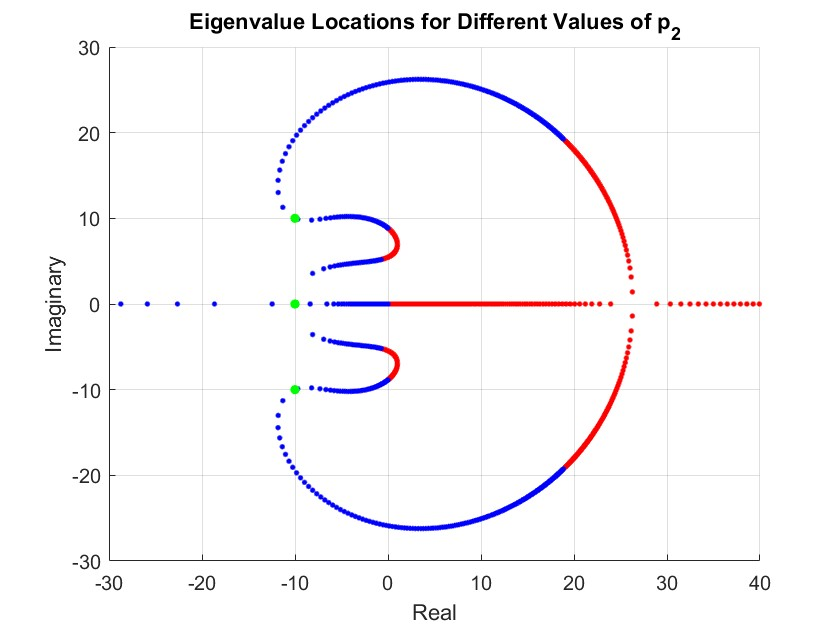
\includegraphics[width=0.6\textwidth]{figures/3.5roots.jpg}
  \caption{Crane root locus for varying $k_2$ only}
  \label{fig:roots3.5}
\end{figure}

\begin{figure}[H]
  \centering
  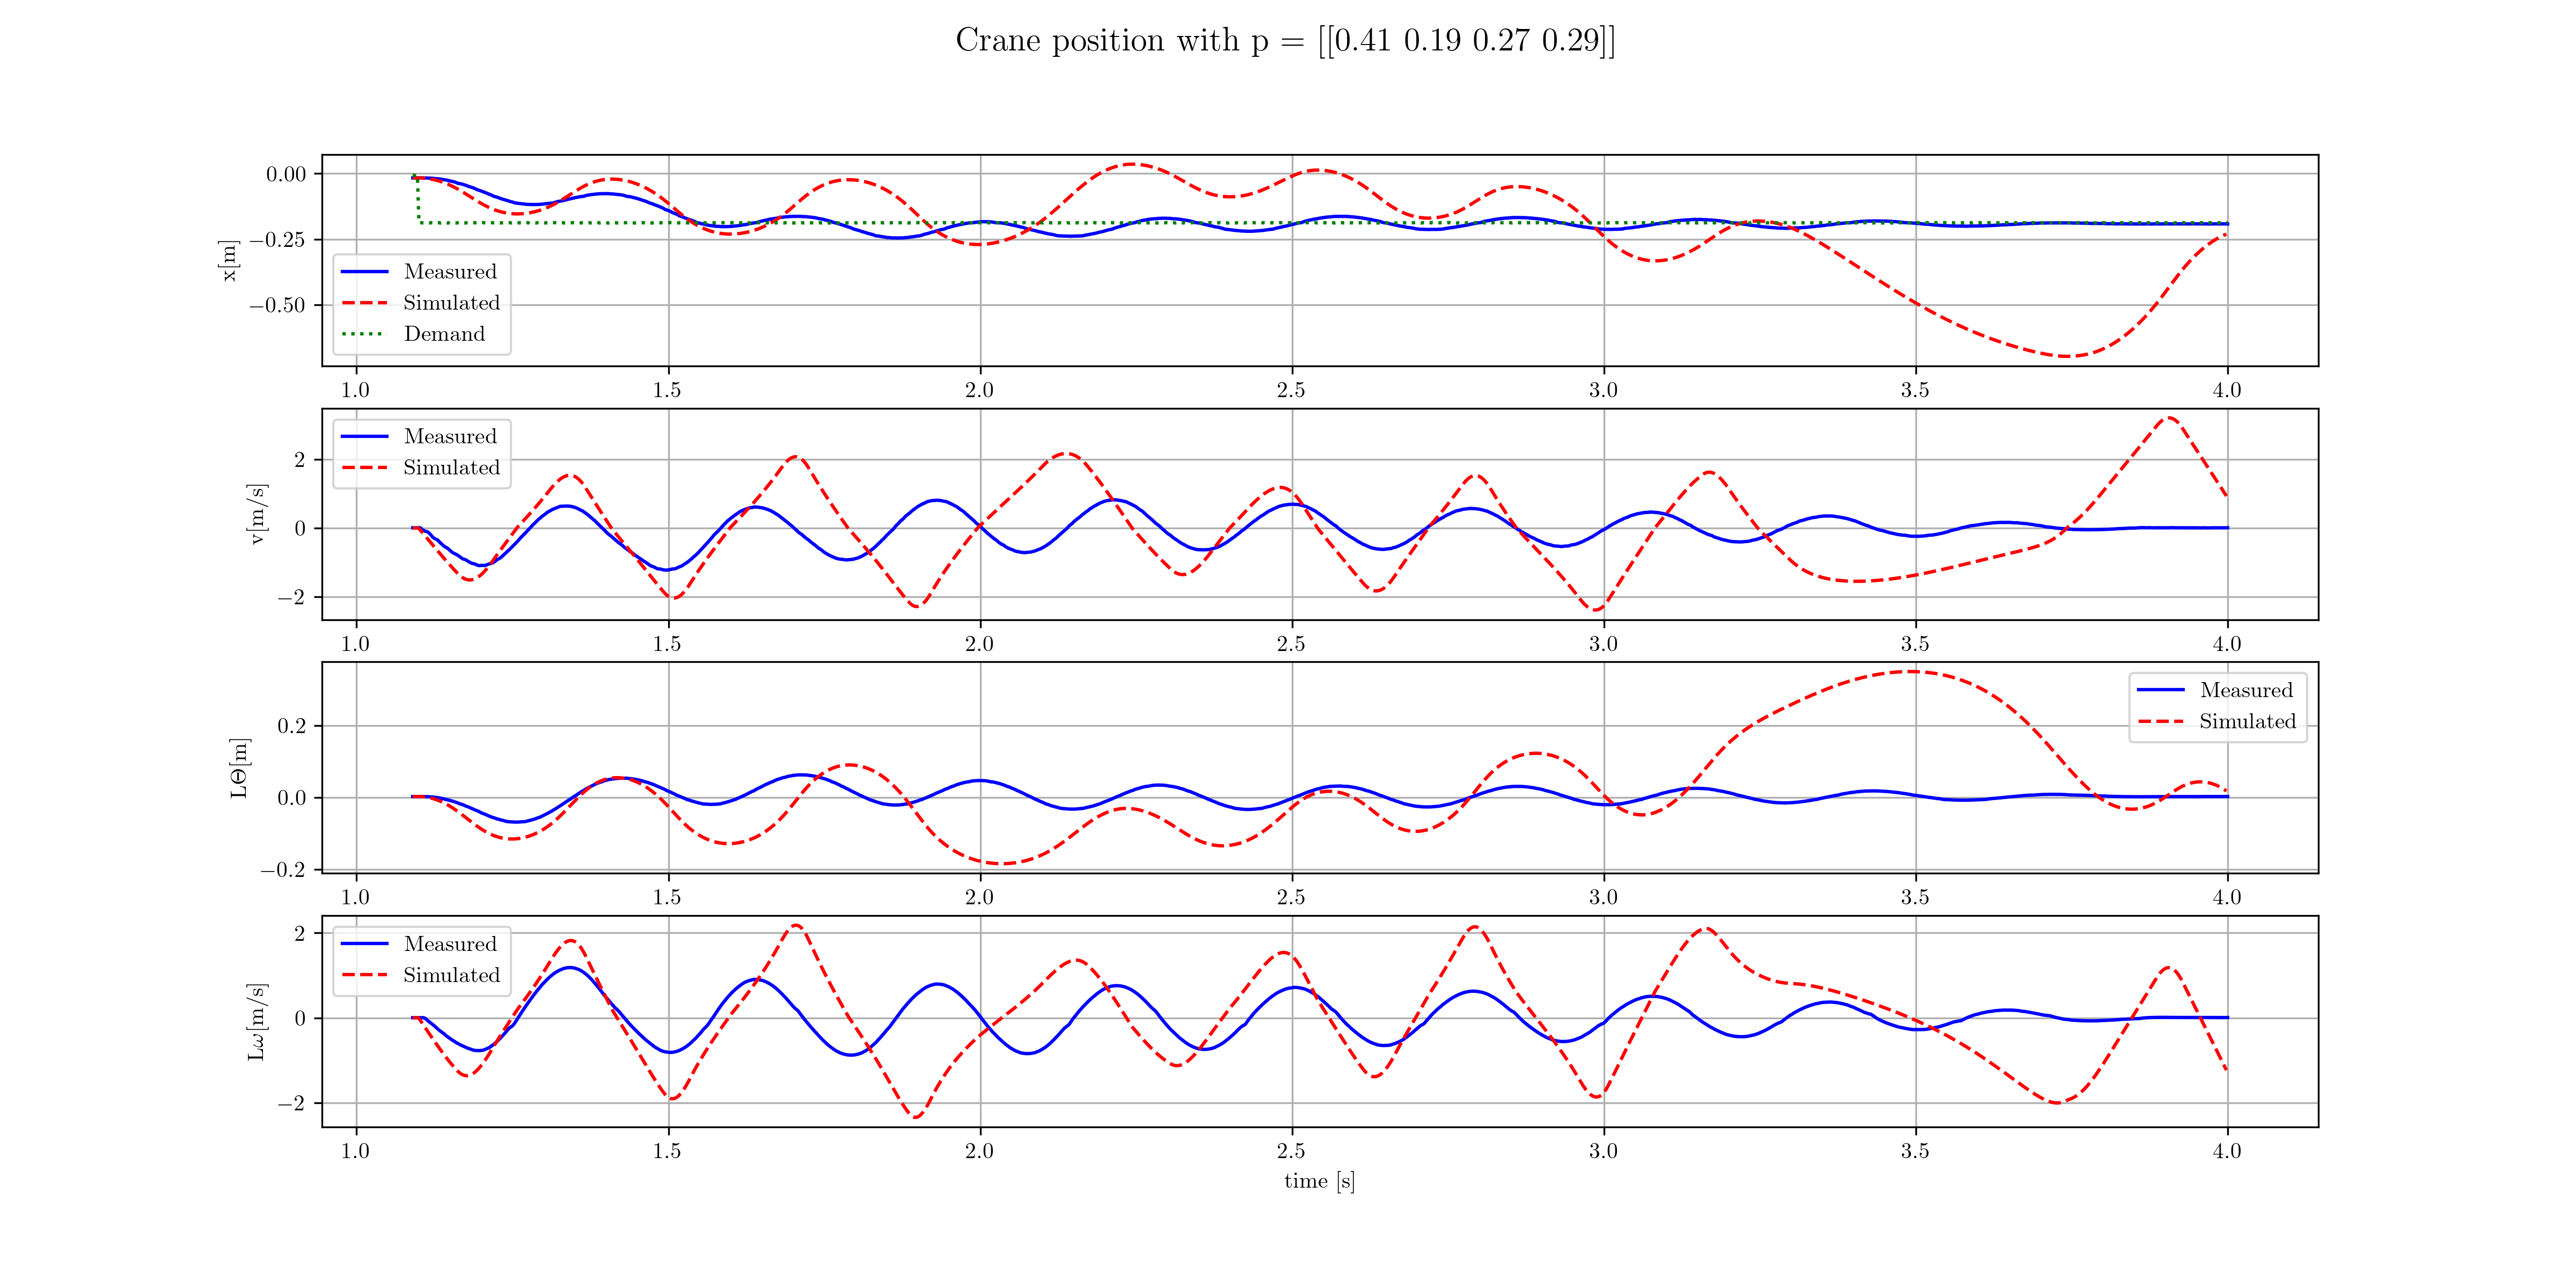
\includegraphics[width=0.99\textwidth]{figures/3.5.png}
  \caption{Limit of stability}
  \label{fig:exp3.5}
\end{figure}

Predicted gain $k_2 =   41.426084064823016$ </br>
Predicted frequency $\hat{\omega} = 4.105928985604413$ Hz

The value of $p_2$ was reduced from 0.46 to 0.19 where the onset of oscillations was observed</br>
Measured Gain $k_2 = 31.35$ </br>
Measured frequency 21.67 rad/s
The amplitude of velocity of the carriage drops to half of the maximum value after 4 cycles, which gives the damping ratio as $\zeta \approx 0.03$

The closed loop pole locations are $[ 4.57476482 \pm 26.11156105j , -1.93649322 \pm 4.95114934j]$ </br>
The first two poles that lie to the right of the imaginary axis suggests that the system should be unstable for this value of $p_2 = 0.19$.


Measurements indicate that the gain $k_2$ for unstability is smaller than expected. </br>

From theory covered in A6 of the appendix, the onset of instability is related to friction in the limit cycles which is not considered in linear theory. </br>
For small oscillations the real system has a large additional damping term from friction, which is why the linear model predicts instability to occur at a higher gain than observed. </br>

At a gain of $p_2 = 0.18$ oscillations occur at larger amplitudes and so according to A6 the additional damping from friction is smaller which causes the system to become unstable. </br> 

\subsection{Inverted Pendulum}

% No Carriage feedback
%% EXPLAIN BEHAVIOUR

% 4.3 pole placement at -omega1
\begin{figure}[H]
  \centering
  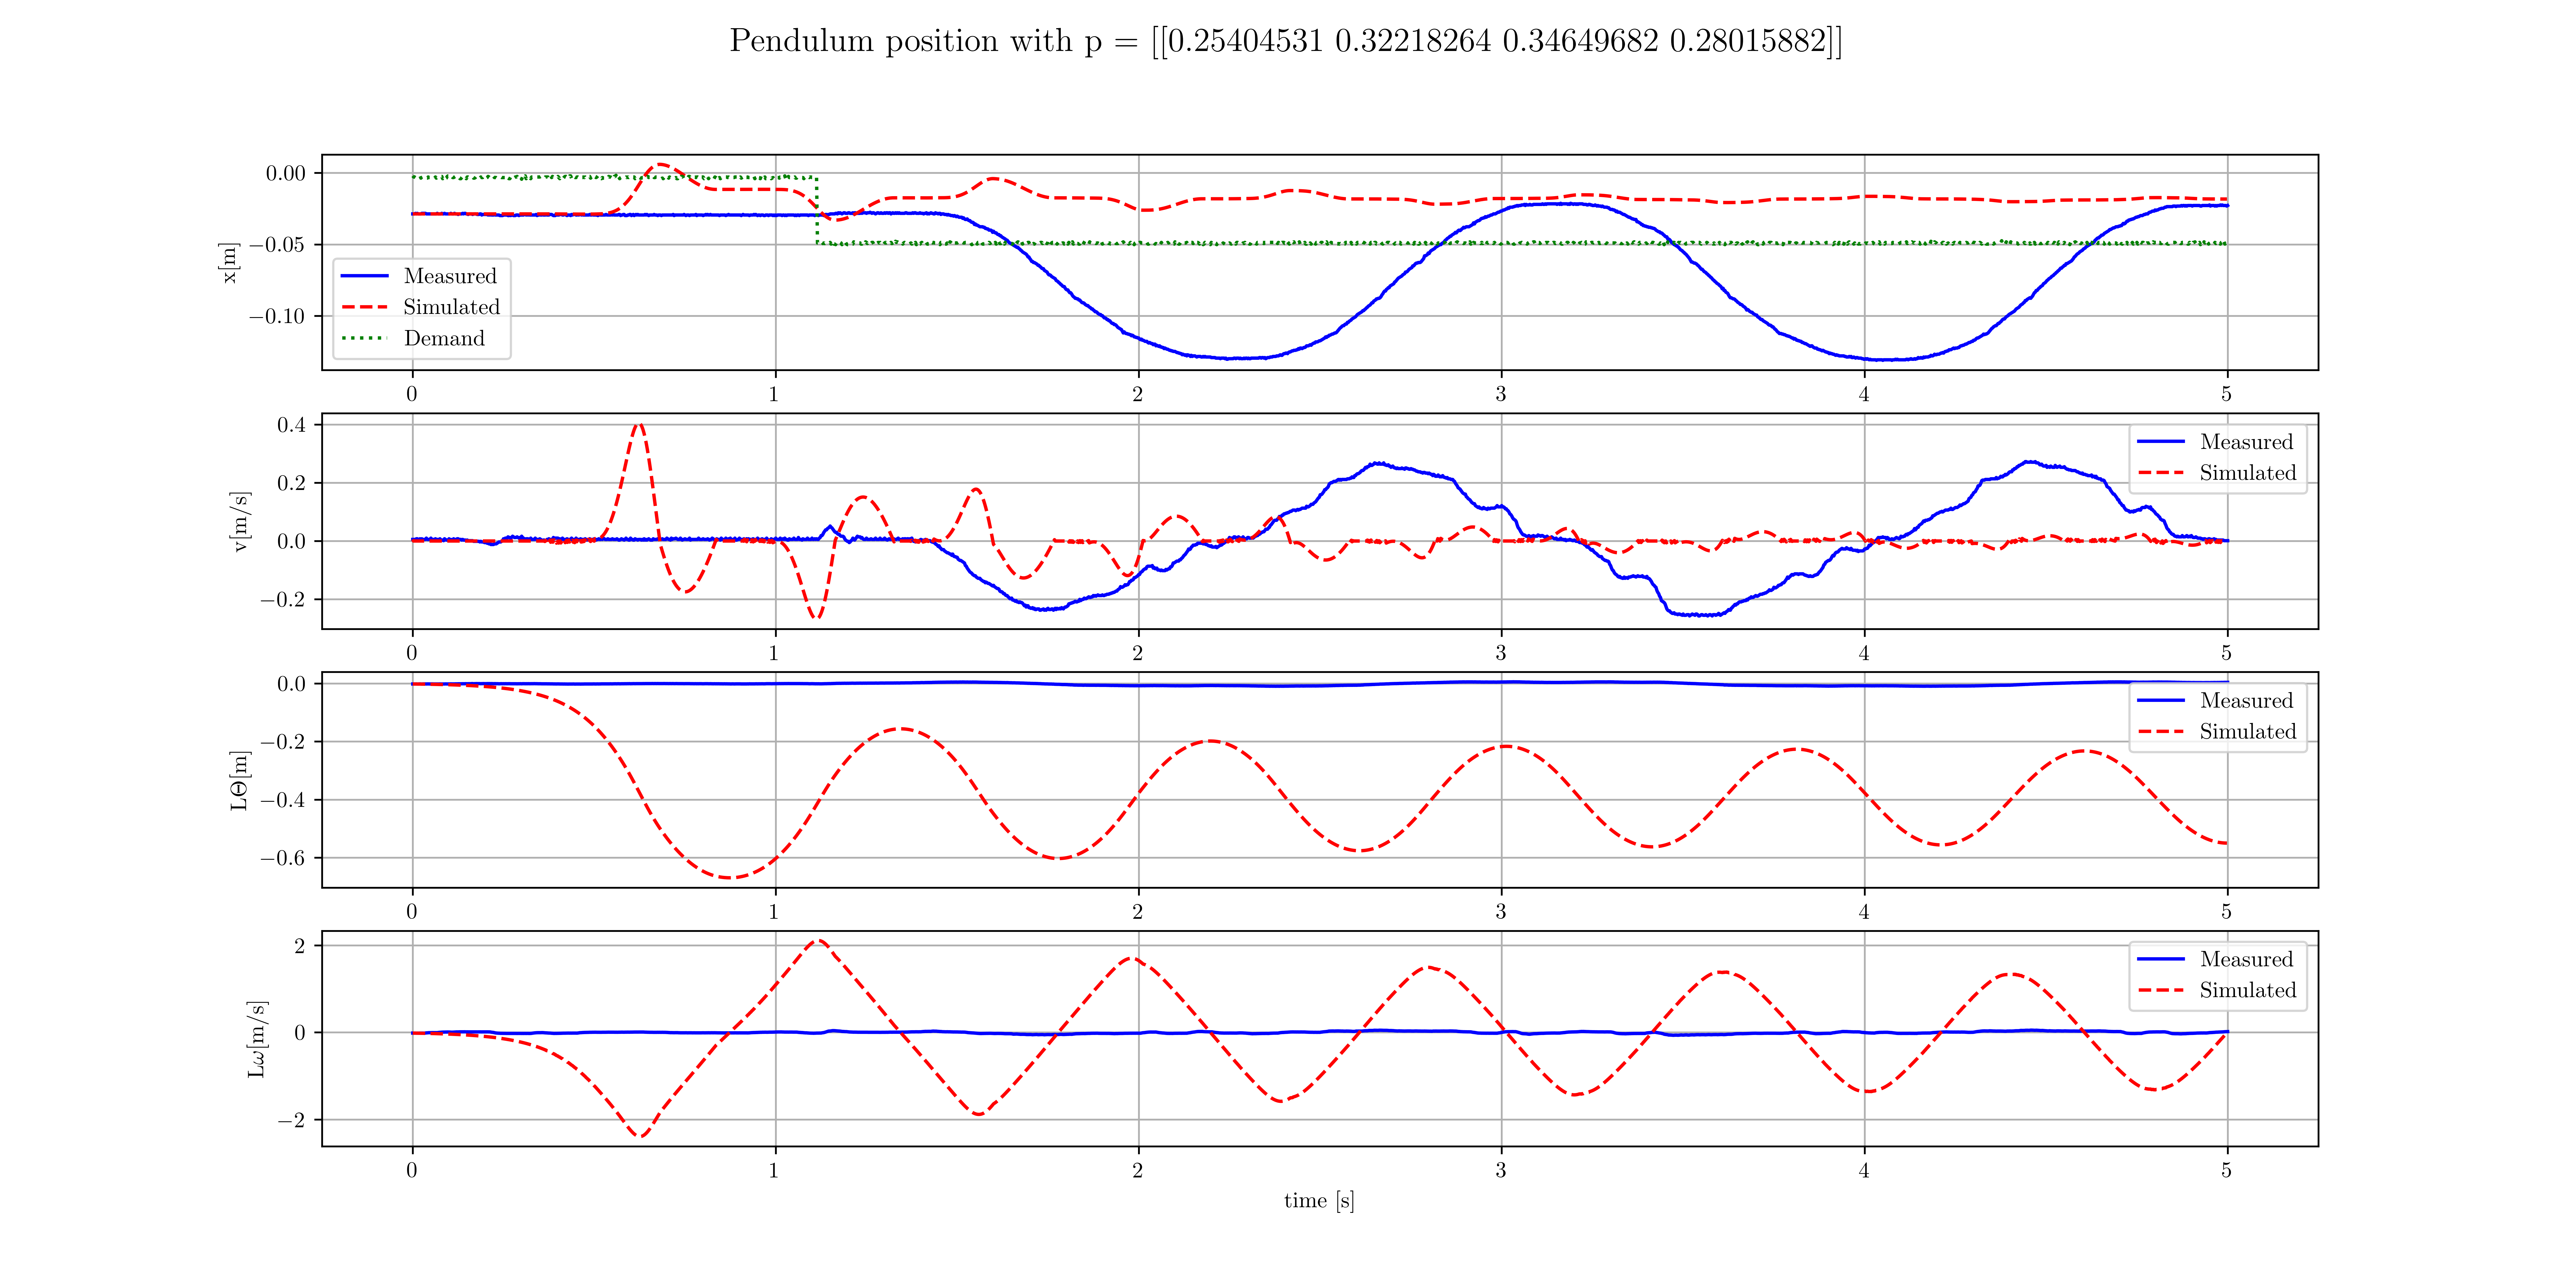
\includegraphics[width=0.99\textwidth]{figures/4.3.png}
  \caption{Inverted pendulum root locus for varying $k_2$ only}
  \label{fig:4.3}
\end{figure}

% 4.4 limit cycles

\begin{figure}[H]
  \centering
  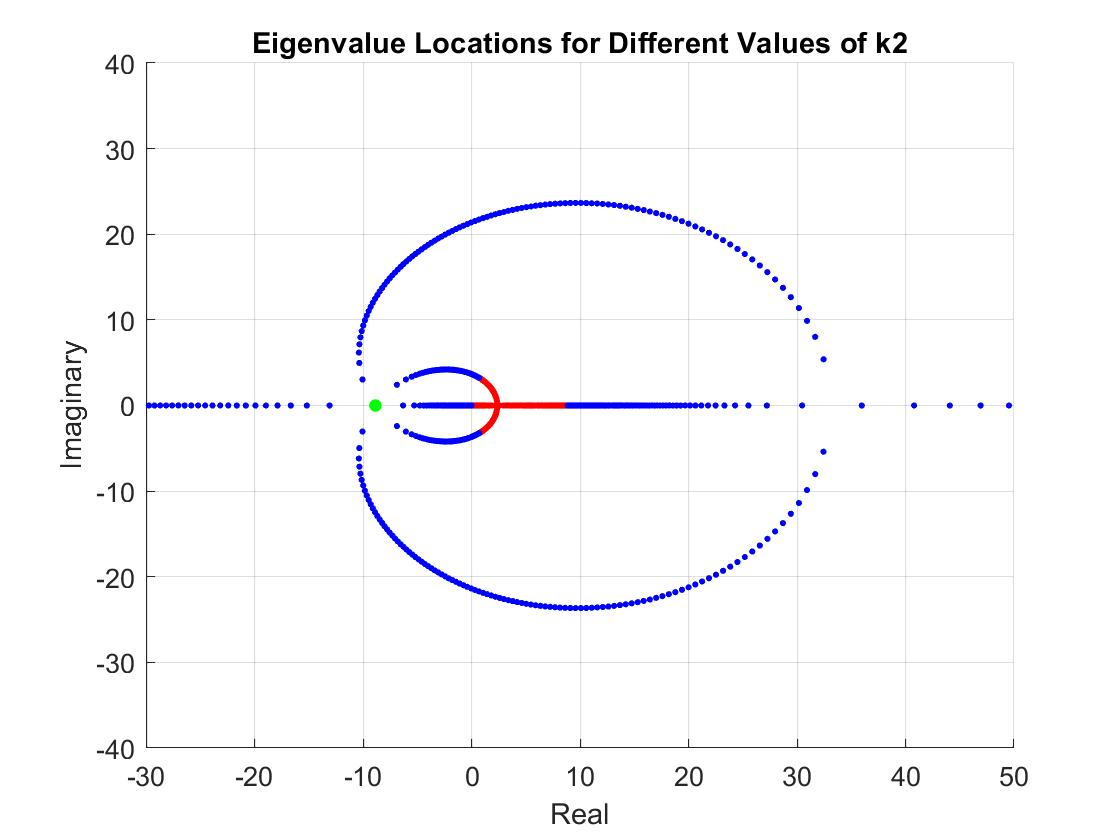
\includegraphics[width=0.6\textwidth]{figures/4.4roots.jpg}
  \caption{Inverted pendulum root locus for varying $k_2$ only}
  \label{fig:roots4.4}
\end{figure}

\begin{figure}[H]
  \centering
  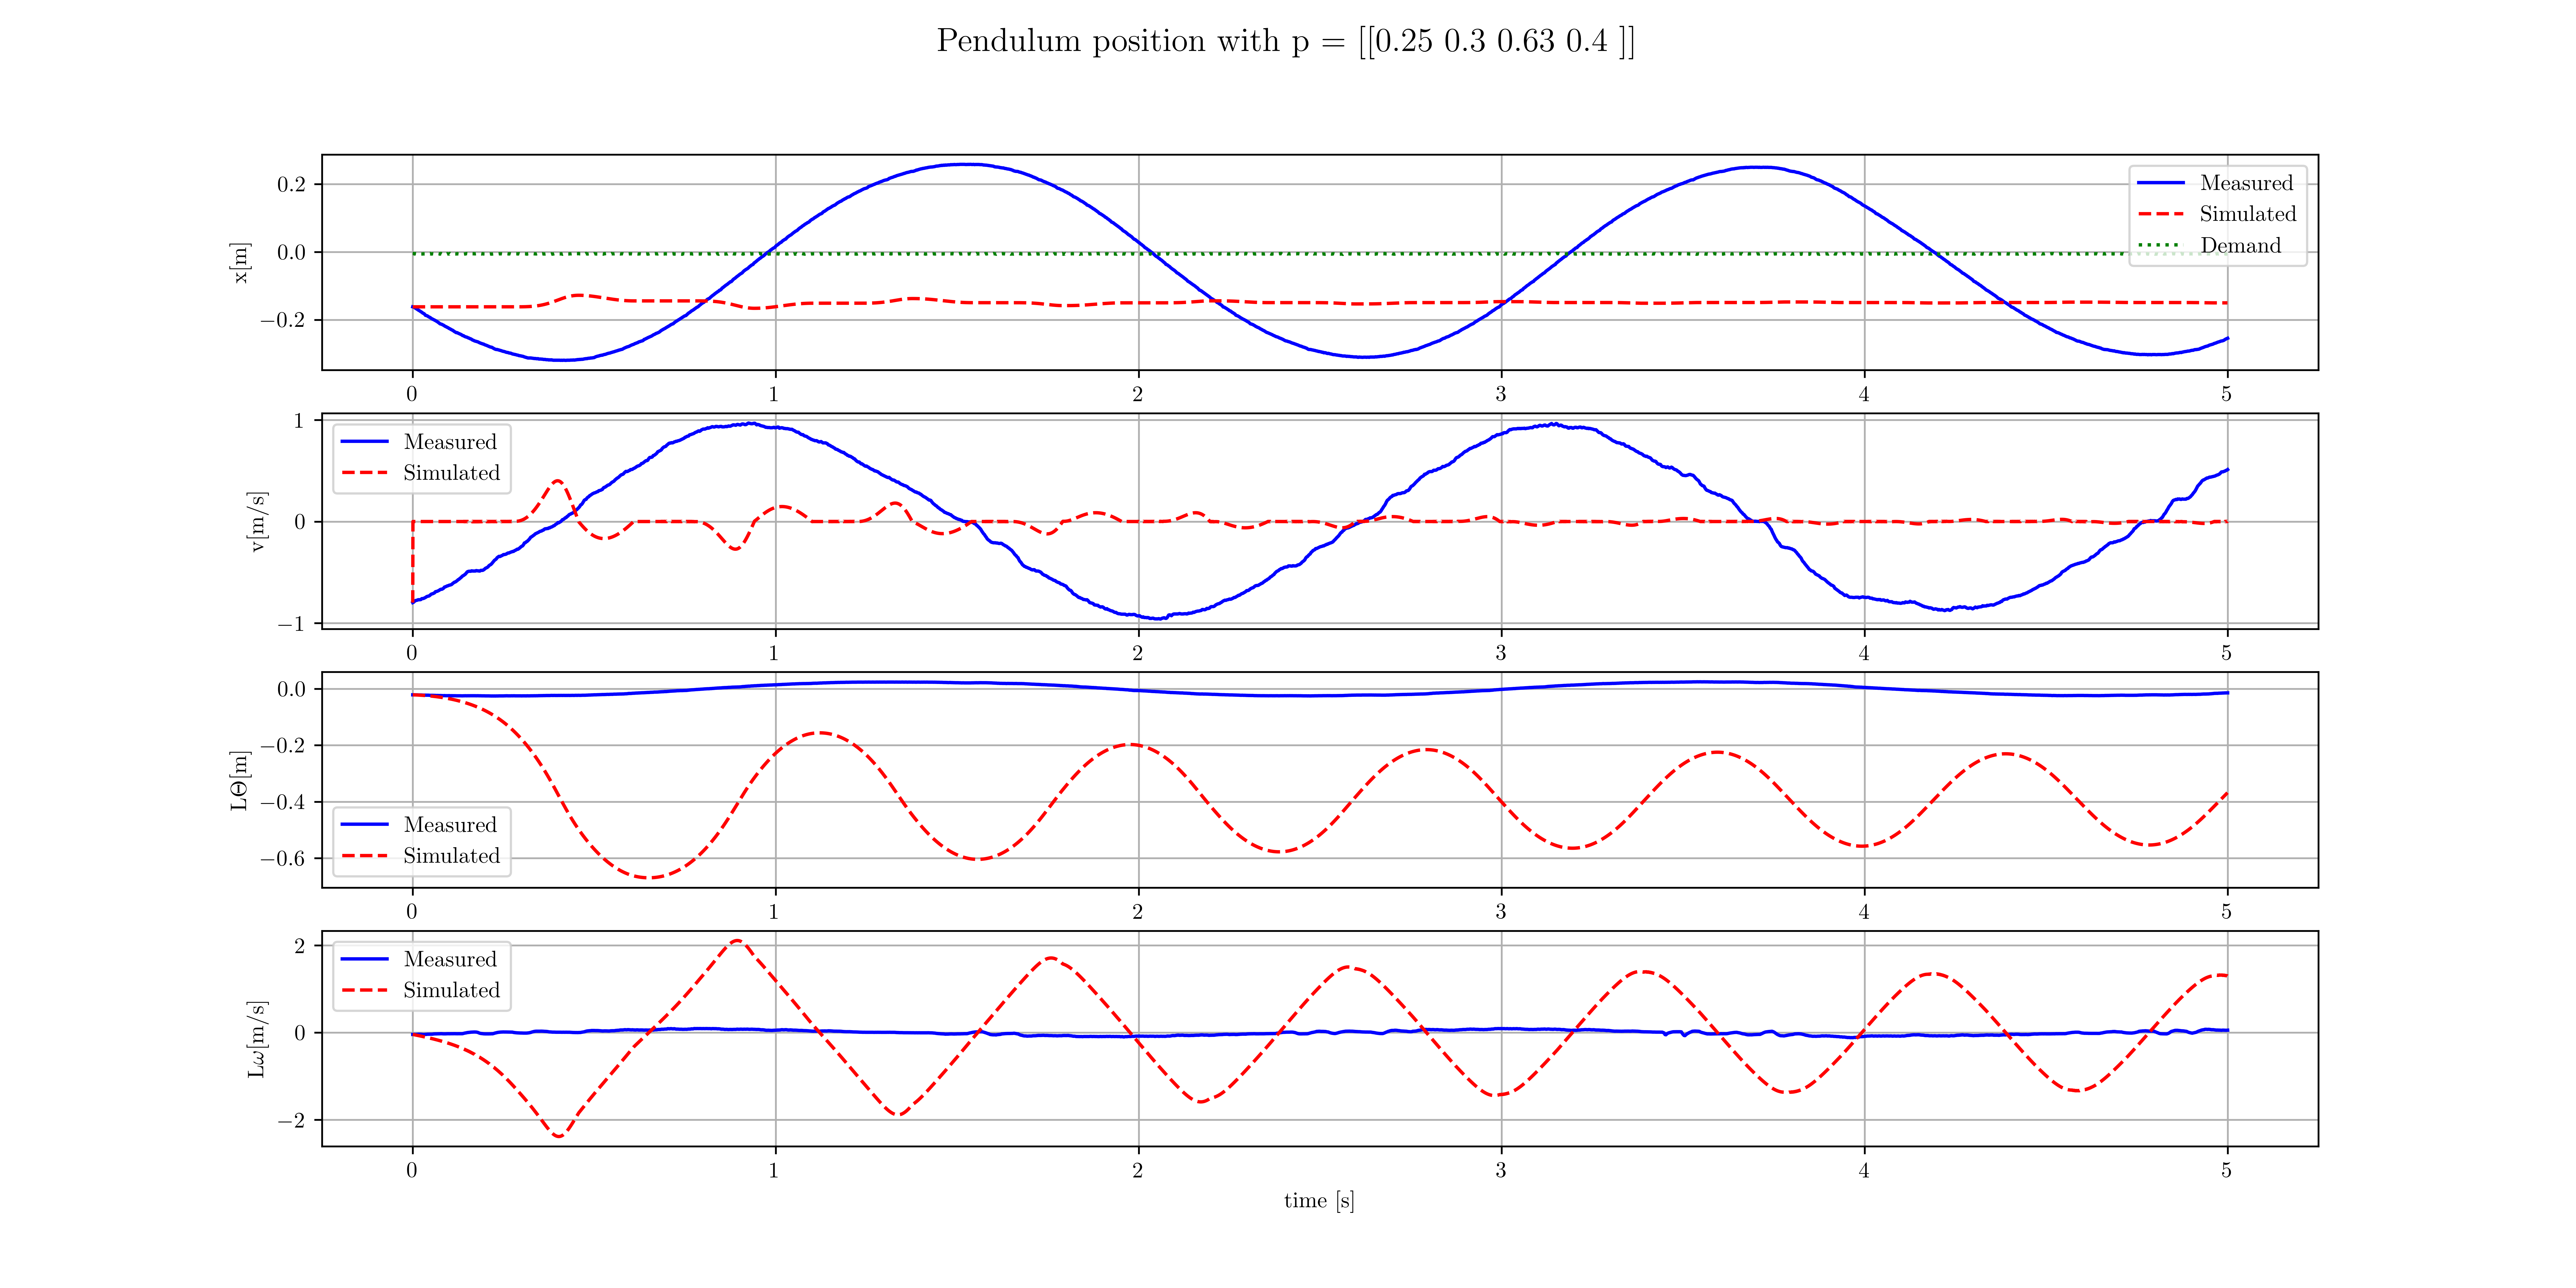
\includegraphics[width=0.99\textwidth]{figures/4.4_lo.png}
  \caption{Inverted pendulum response at minimum $k_2 = $ for stability}
  \label{fig:roots4.4_lo}
\end{figure}

The value of $p_2 = 0.3$ was found for large oscillations.
This can be seen in the poles $-1.27029093 \pm 2.37834982j$
These have a small imaginary component and so have a lower frequency, as observed.
The value of damping is also small which is given by the real part.

\begin{figure}[H]
  \centering
  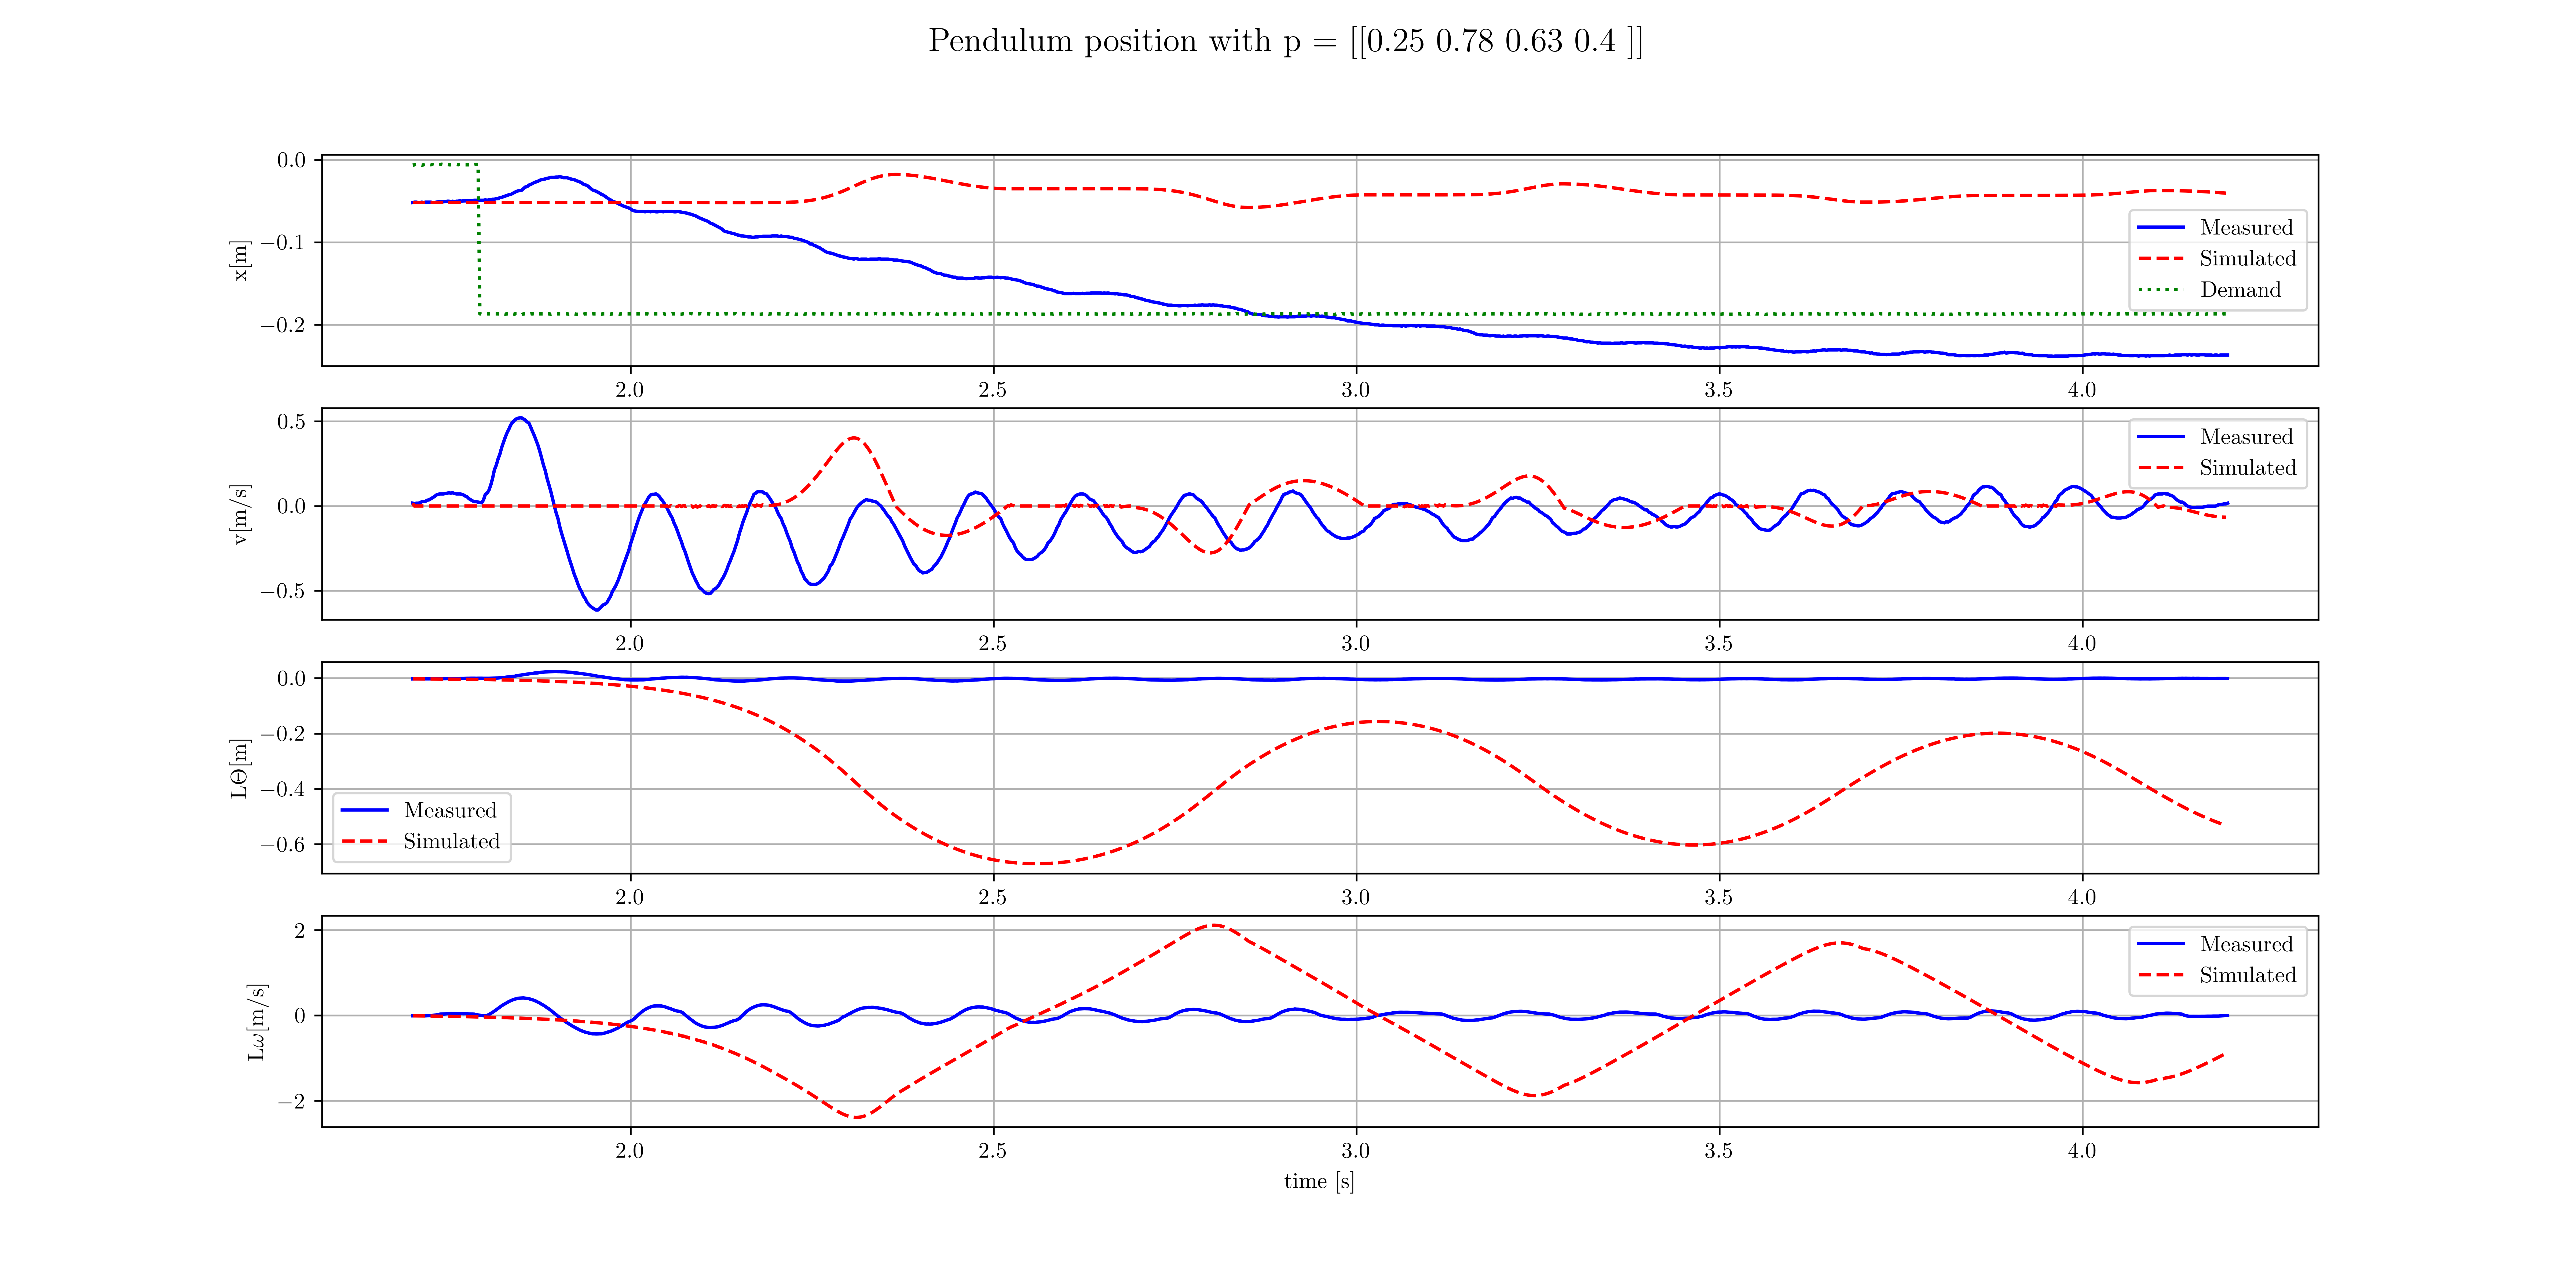
\includegraphics[width=0.99\textwidth]{figures/4.4_hi.png}
  \caption{Inverted pendulum response at maximum $k_2 = $ for stability}
  \label{fig:roots4.4_hi}
\end{figure}

Value of $p_2$ for at the onset of instability: 0.78
The carriage velocity amplitude halves after 7 cycles giving a damping ratio of $\zeta \approx 0.016$
The frequency of carriage velocity is calculated to be about 44 rad/s
This gives calculated poles of $-0.704 \pm 44j$

The corresponding poles of the system are $-4.07147154 \pm 30.42971361j$
This shows that the damping is higher than expected 

\section{Discussion}

currently in the results


\section{Conclusion}


\newpage
\section{Appendix}

\begin{align}
  \left( 1 + \frac{M}{m} + \frac{I}{ma^2} \right) \ddot{x} &= \frac{T}{ma} - \frac{F}{m}\text{sgn}(\dot{x}) - l\sin\phi . \ddot{\phi} - l\cos\phi . \dot{\phi}^2 \\
   - l \ddot{\phi} &= \sin\phi \ddot{x} - g\cos\phi
\end{align}

Crane closed loop transfer function
\begin{equation}
  \mathbf{C} (s\mathbf{I} - \mathbf{A} + \mathbf{KB}) ^{-1} \mathbf{B} = \left[\begin{matrix}\frac{617.283950617284 \left(\omega_{1}^{2} + s^{2}\right)}{k_{1} \omega_{1}^{2} + k_{1} s^{2} + k_{2} \omega_{1}^{2} s + k_{2} s^{3} + k_{3} s^{2} + k_{4} s^{3} + \omega_{0}^{2} s^{2} + s^{4}}\\\frac{165.185185185185 s \left(\omega_{1}^{2} + s^{2}\right)}{k_{1} \omega_{1}^{2} + k_{1} s^{2} + k_{2} \omega_{1}^{2} s + k_{2} s^{3} + k_{3} s^{2} + k_{4} s^{3} + \omega_{0}^{2} s^{2} + s^{4}}\\\frac{1256.2962962963 s^{2}}{k_{1} \omega_{1}^{2} + k_{1} s^{2} + k_{2} \omega_{1}^{2} s + k_{2} s^{3} + k_{3} s^{2} + k_{4} s^{3} + \omega_{0}^{2} s^{2} + s^{4}}\\- \frac{126.41975308642 s^{3}}{k_{1} \omega_{1}^{2} + k_{1} s^{2} + k_{2} \omega_{1}^{2} s + k_{2} s^{3} + k_{3} s^{2} + k_{4} s^{3} + \omega_{0}^{2} s^{2} + s^{4}}\end{matrix}\right]
\end{equation}

Inverted pendulum closed loop transfer function

\begin{equation}
  \mathbf{C} (s\mathbf{I} - \mathbf{A} + \mathbf{KB}) ^{-1} \mathbf{B} = \left[\begin{matrix}\frac{617.283950617284 \left(- \omega_{1}^{2} + s^{2}\right)}{- k_{1} \omega_{1}^{2} + k_{1} s^{2} - k_{2} \omega_{1}^{2} s + k_{2} s^{3} + k_{3} s^{2} + k_{4} s^{3} - \omega_{0}^{2} s^{2} + s^{4}}\\\frac{165.185185185185 s \left(- \omega_{1}^{2} + s^{2}\right)}{- k_{1} \omega_{1}^{2} + k_{1} s^{2} - k_{2} \omega_{1}^{2} s + k_{2} s^{3} + k_{3} s^{2} + k_{4} s^{3} - \omega_{0}^{2} s^{2} + s^{4}}\\\frac{1256.2962962963 s^{2}}{- k_{1} \omega_{1}^{2} + k_{1} s^{2} - k_{2} \omega_{1}^{2} s + k_{2} s^{3} + k_{3} s^{2} + k_{4} s^{3} - \omega_{0}^{2} s^{2} + s^{4}}\\- \frac{126.41975308642 s^{3}}{- k_{1} \omega_{1}^{2} + k_{1} s^{2} - k_{2} \omega_{1}^{2} s + k_{2} s^{3} + k_{3} s^{2} + k_{4} s^{3} - \omega_{0}^{2} s^{2} + s^{4}}\end{matrix}\right]
\end{equation}

% bibliography
\newpage
\begin{thebibliography}{9}

\end{thebibliography}

\end{document}